\section{Results}
\label{sec:results}

This chapter presents the empirical findings in four stages. Section~\ref{sec:descriptive} establishes the geographic structure of treatment variation. Section~\ref{sec:pooled_results} reports the primary pooled event-study estimates for wages and employment. Section~\ref{sec:cohort_results} decomposes these effects using the Duflo-style age-cohort design. Section~\ref{sec:heterogeneity} explores distributional impacts by gender and ethnicity, and Section~\ref{sec:robustness_results} reports robustness checks.

Before turning to the estimates, it is useful to distinguish clearly between what is identified and what is more tentative. The primary causal objects in this chapter are the within-stratum group-time ATTs for Low-Dose and High-Dose microregions estimated under the not-yet-treated parallel trends assumption. By contrast, direct comparisons between the Low-Dose and High-Dose paths require stronger assumptions and are therefore interpreted as suggestive patterns rather than as clean causal dose-response effects.

\subsection{Geographic Distribution of Treatment Intensity}
\label{sec:descriptive}

Figure~\ref{fig:heatmap} displays the spatial distribution of cumulative ProUni scholarship density ($D_{r,2019}$) across Brazil's 558 microregions. The map reveals a pronounced geographic concentration: the South and Southeast---particularly the S\~ao Paulo metropolitan corridor, Porto Alegre, and Belo Horizonte---exhibit the highest treatment intensities, while the Amazon basin and parts of the Northeast received substantially lower exposure. This pattern is consistent with the unequal distribution of pre-existing private HEI infrastructure, although the map by itself does not establish exogeneity.

\begin{figure}[ht]
\centering
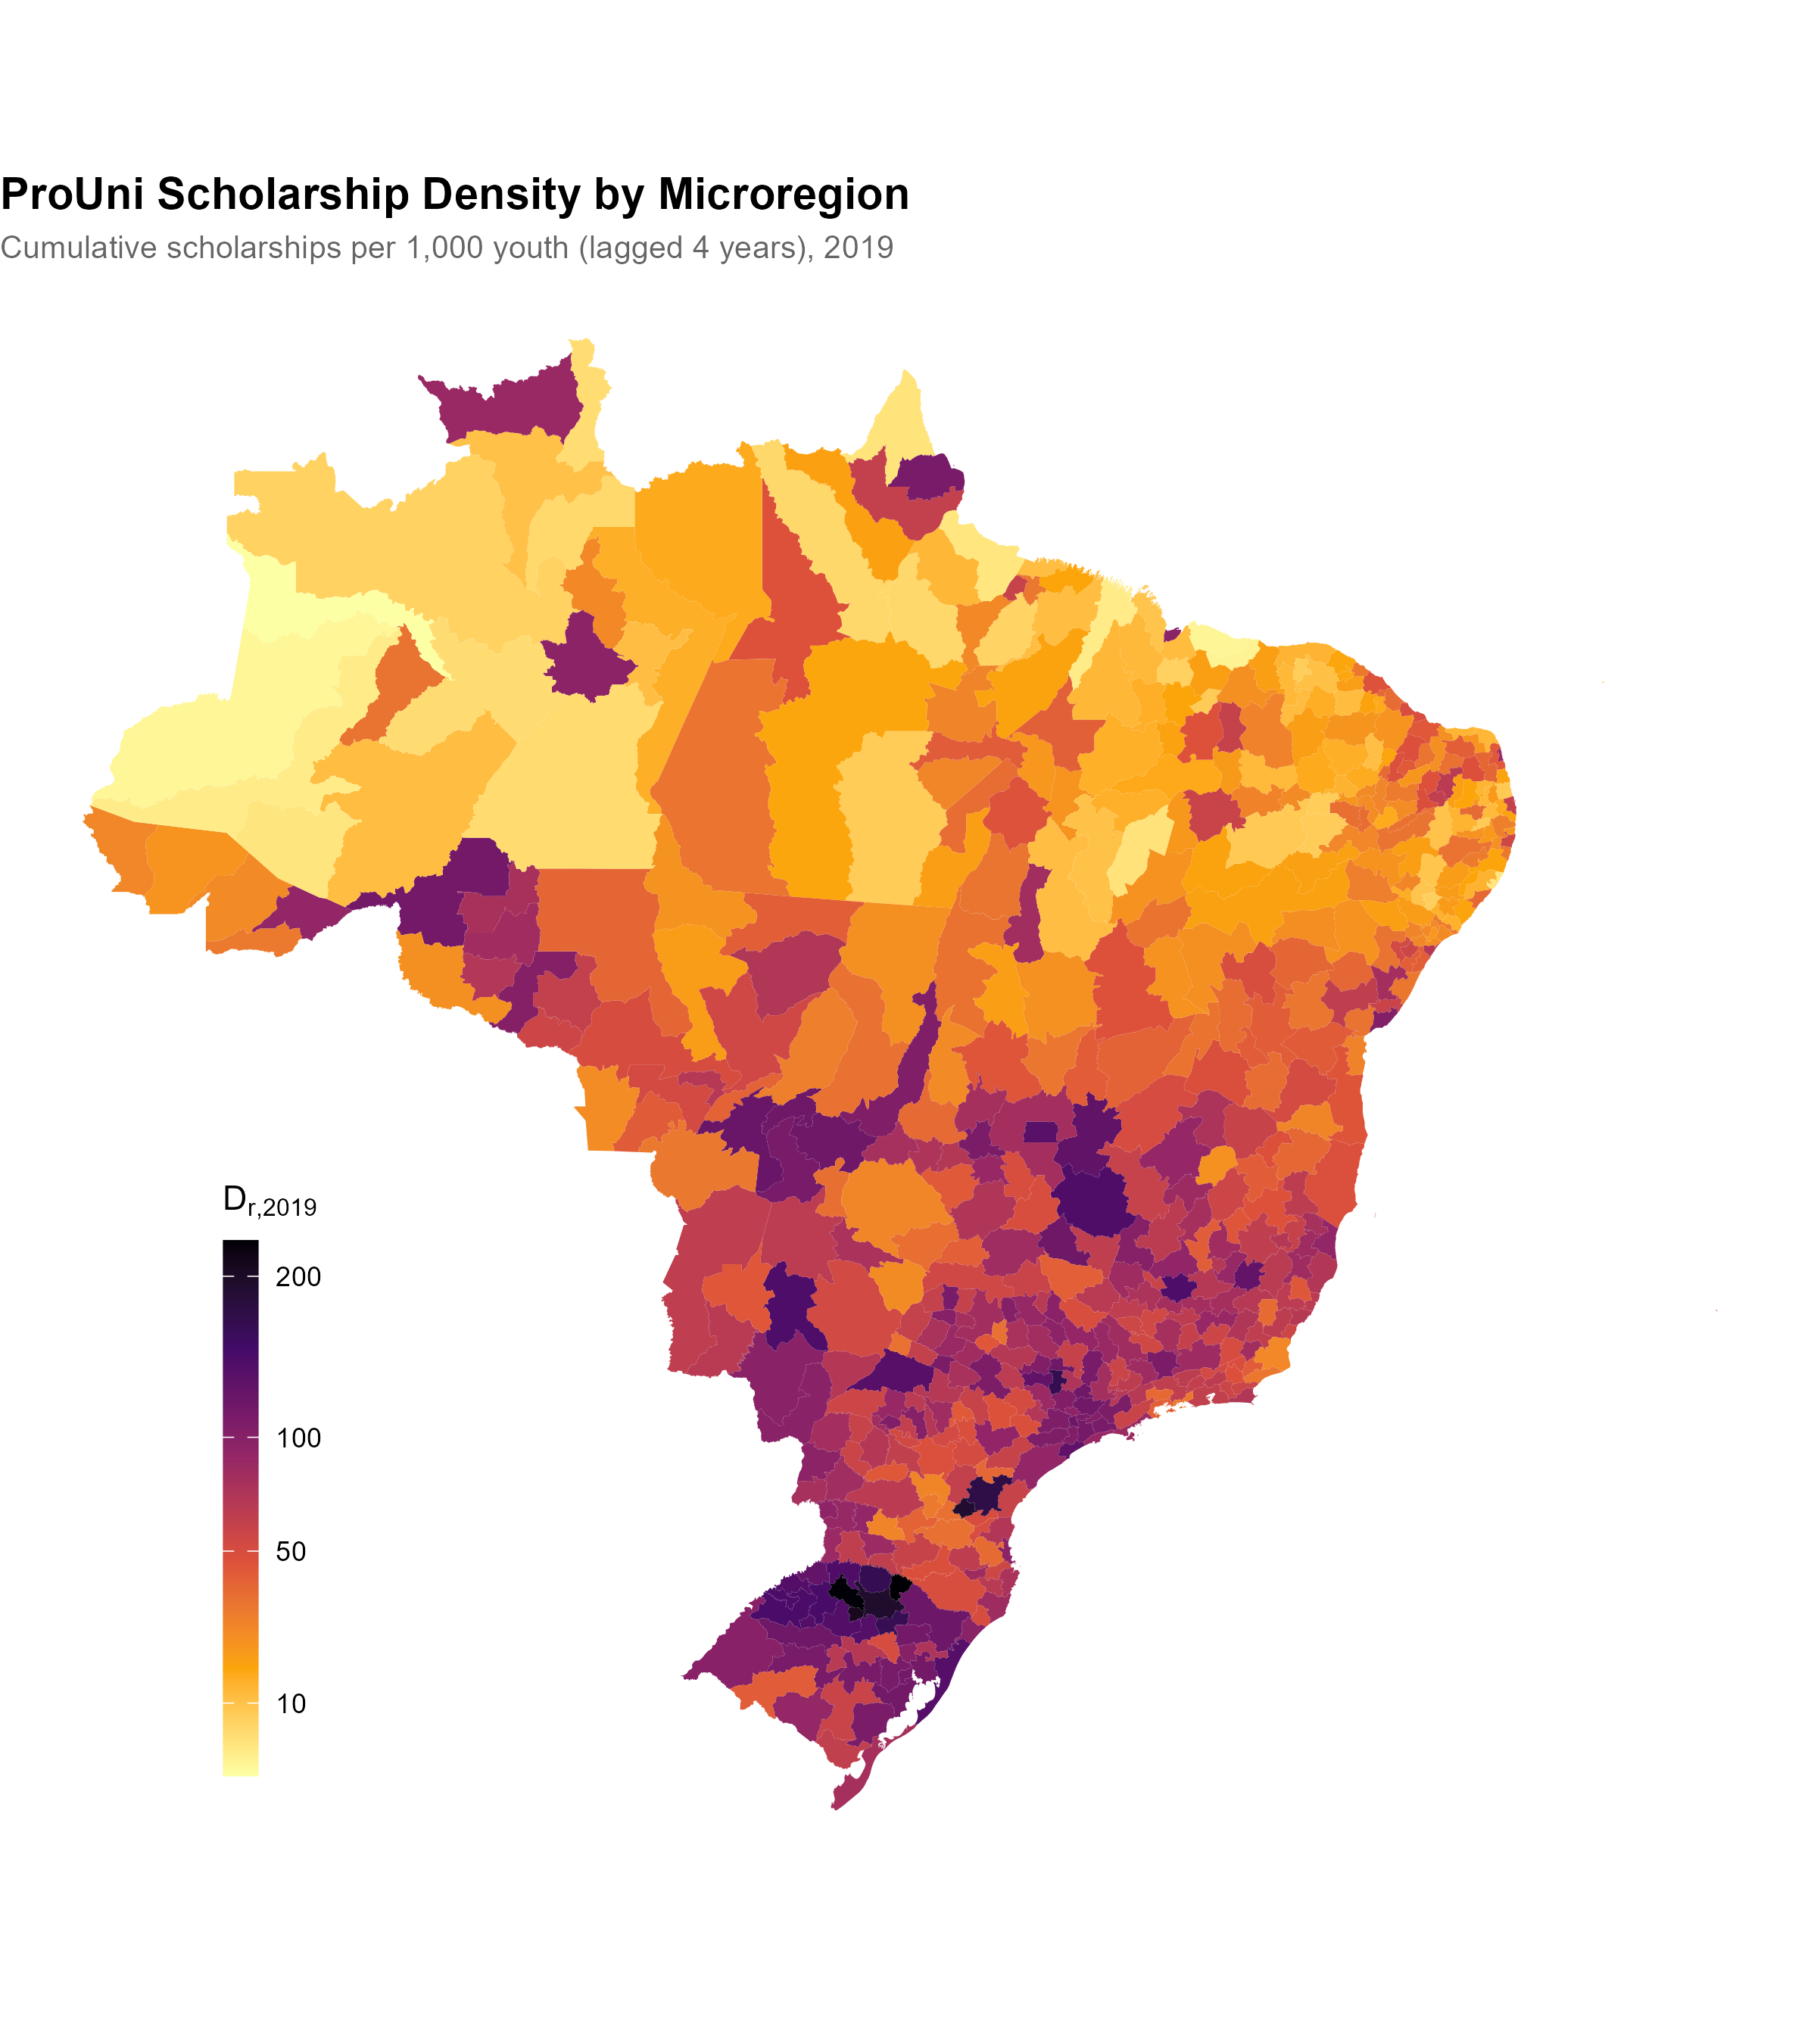
\includegraphics[width=0.75\textwidth]{Figures/fig_map_dose_continuous.png}
\caption{\textbf{ProUni Scholarship Density by Microregion, 2019.} Cumulative scholarships per 1,000 youth (aged 18--24), lagged four years. Color intensity follows a square-root scale to accommodate the right-skewed distribution.}
\label{fig:heatmap}
\end{figure}

Table~\ref{tab:att_baseline} reports summary statistics by dose bin. High-Dose microregions are characterized by larger youth populations and higher absolute treatment intensities, having crossed the treatment threshold earlier (median year 2012) than their Low-Dose counterparts (median year 2017). These differences reinforce the need to interpret cross-dose contrasts cautiously, since heavily exposed markets are not simply scaled-up versions of lightly exposed ones.

\begin{table}[ht]
\centering
\caption{\textbf{Summary Statistics by Dose Bin (2019)}}
\label{tab:att_baseline}
\begin{tabular}{lcccc}
\hline
\textbf{Dose Bin} & \textbf{N. Regions} & \textbf{Avg. Youth Pop.} & \textbf{Avg. Density} & \textbf{Median Treatment Yr} \\
\hline
Low & 167 & 27,689 & 33.74 & 2017 \\
High & 140 & 74,598 & 107.43 & 2012 \\
\hline
\end{tabular}
\end{table}

\subsection{Pooled Event-Study Estimates}
\label{sec:pooled_results}

\subsubsection{Wages: Baseline Reduced-Form Evidence}

Figure~\ref{fig:dose_response} presents the baseline wage event studies. The dynamic estimates suggest a divergence between Low-Dose and High-Dose microregions after treatment onset, but the safest interpretation remains within each stratum rather than between strata.

\begin{figure}[ht]
\centering
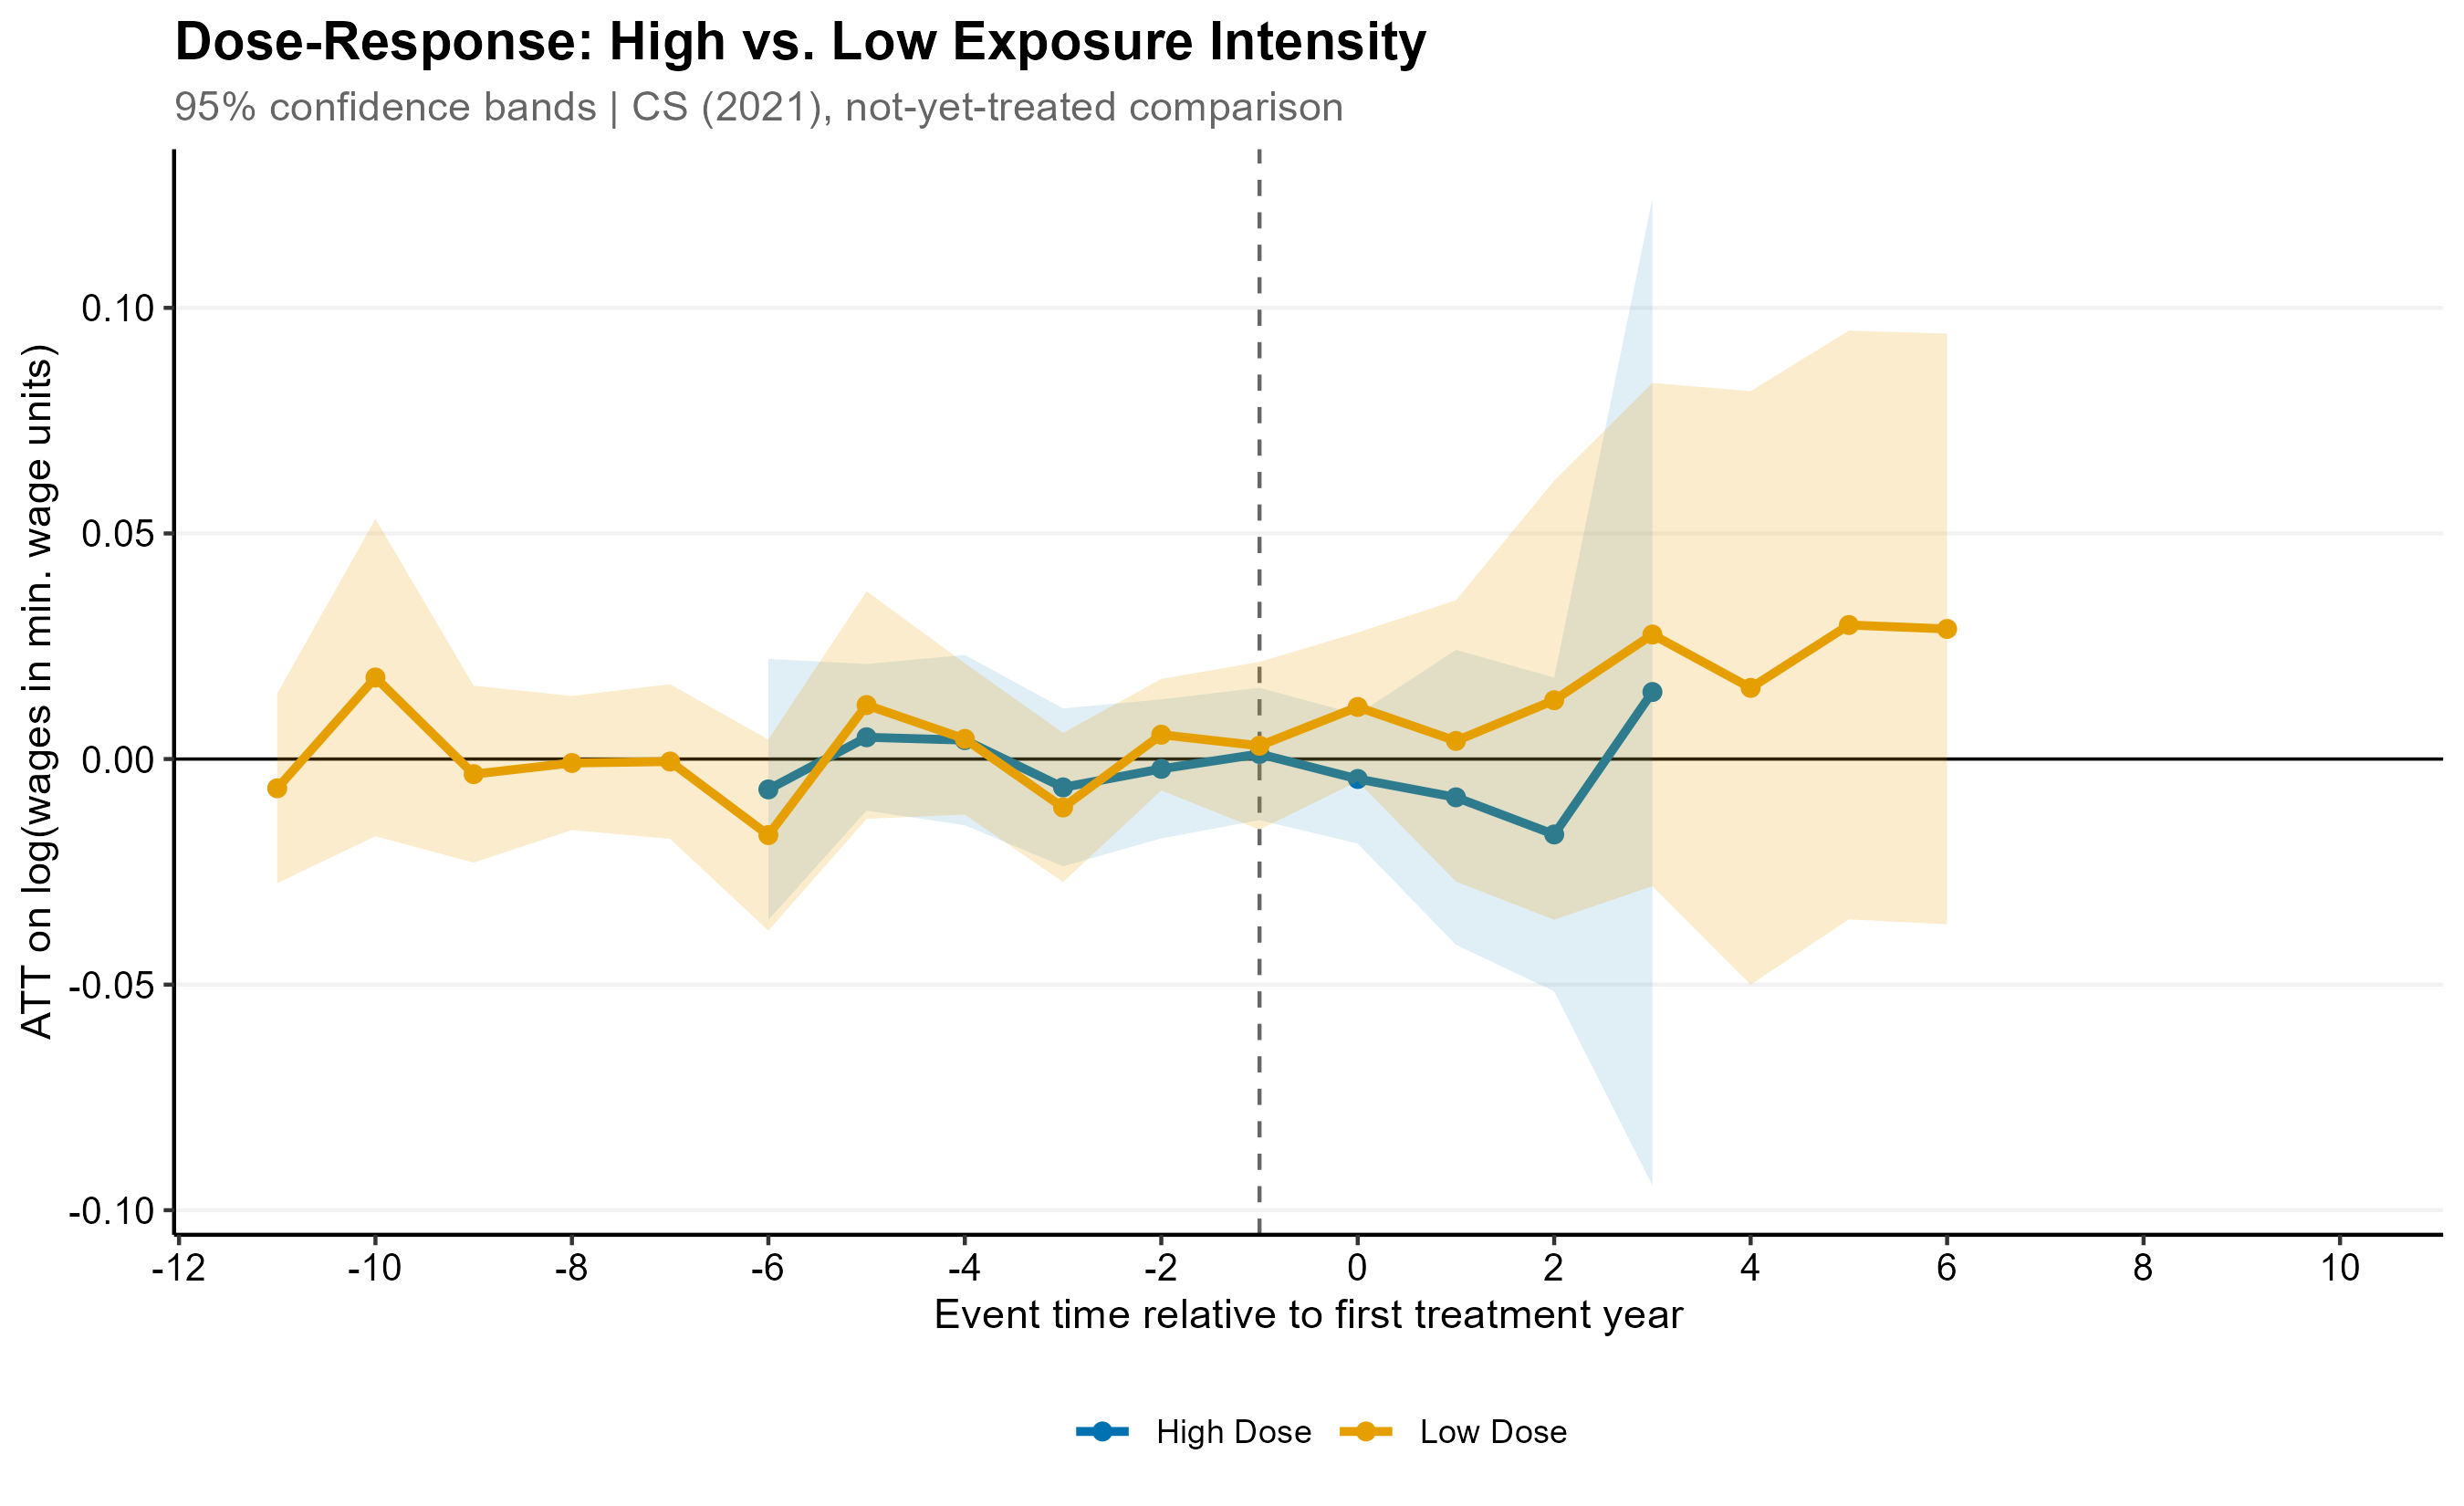
\includegraphics[width=0.85\textwidth]{Figures/fig_1_mechanism_dose.png}
\caption{\textbf{Dose-Response: High vs.\ Low Exposure Intensity.} Dynamic ATT estimates from \citeA{CallawaySantAnna2021}, aggregated via \texttt{aggte(type = ``dynamic'')}. Shaded regions denote 95\% simultaneous confidence bands from the multiplier bootstrap. The dashed vertical line marks $e = -1$, the last pre-treatment period.}
\label{fig:dose_response}
\end{figure}

Three features of Figure~\ref{fig:dose_response} merit emphasis. First, pre-treatment coefficients ($e < 0$) for both dose bins fluctuate around zero, with no obvious systematic drift. Consistent with that visual impression, the joint Wald test fails to reject the null of zero pre-trends at conventional levels for both specifications ($p = 0.359$ for Low Dose; $p = 0.916$ for High Dose). This supports the identifying assumption, although non-rejection should not be read as proof that the assumption holds exactly.

Second, the Low-Dose event study displays a gradually increasing post-treatment trajectory, reaching roughly 2.5--3.0\% by event time $e = 5$--$6$. The overall simple ATT estimate for the Low-Dose bin is $1.28\%$ ($SE = 0.0128$). The estimate is imprecise at conventional levels, but its sign and magnitude are economically meaningful for a reduced-form effect measured on the average wage of all formal workers aged 22--35 within a microregion. In the Doubly Robust specification (Table~\ref{tab:master_summary}), the estimate rises to $2.59\%$ ($SE = 0.0145$, $p < 0.10$), suggesting that the positive low-dose pattern is not driven purely by raw compositional differences.

Third, the High-Dose estimates remain close to zero throughout the post-treatment window. The overall simple ATT is $-0.70\%$ ($SE = 0.0074$). On its own, this pattern is consistent with attenuation of wage gains in heavily exposed markets, but it does not by itself isolate a causal saturation mechanism. As shown below, the high-dose penalty is sensitive to controls for macroeconomic geography, so the evidence for saturation should be read as suggestive rather than definitive.

\subsubsection{Employment: Extensive Margin}

Figure~\ref{fig:employment} reports the employment-margin estimates. Both dose bins show near-zero effects for the first four post-treatment years. The overall ATT on log formal employment is $1.82\%$ ($SE = 0.0332$) for Low Dose and $0.65\%$ ($SE = 0.0396$) for High Dose.

\begin{figure}[ht]
\centering
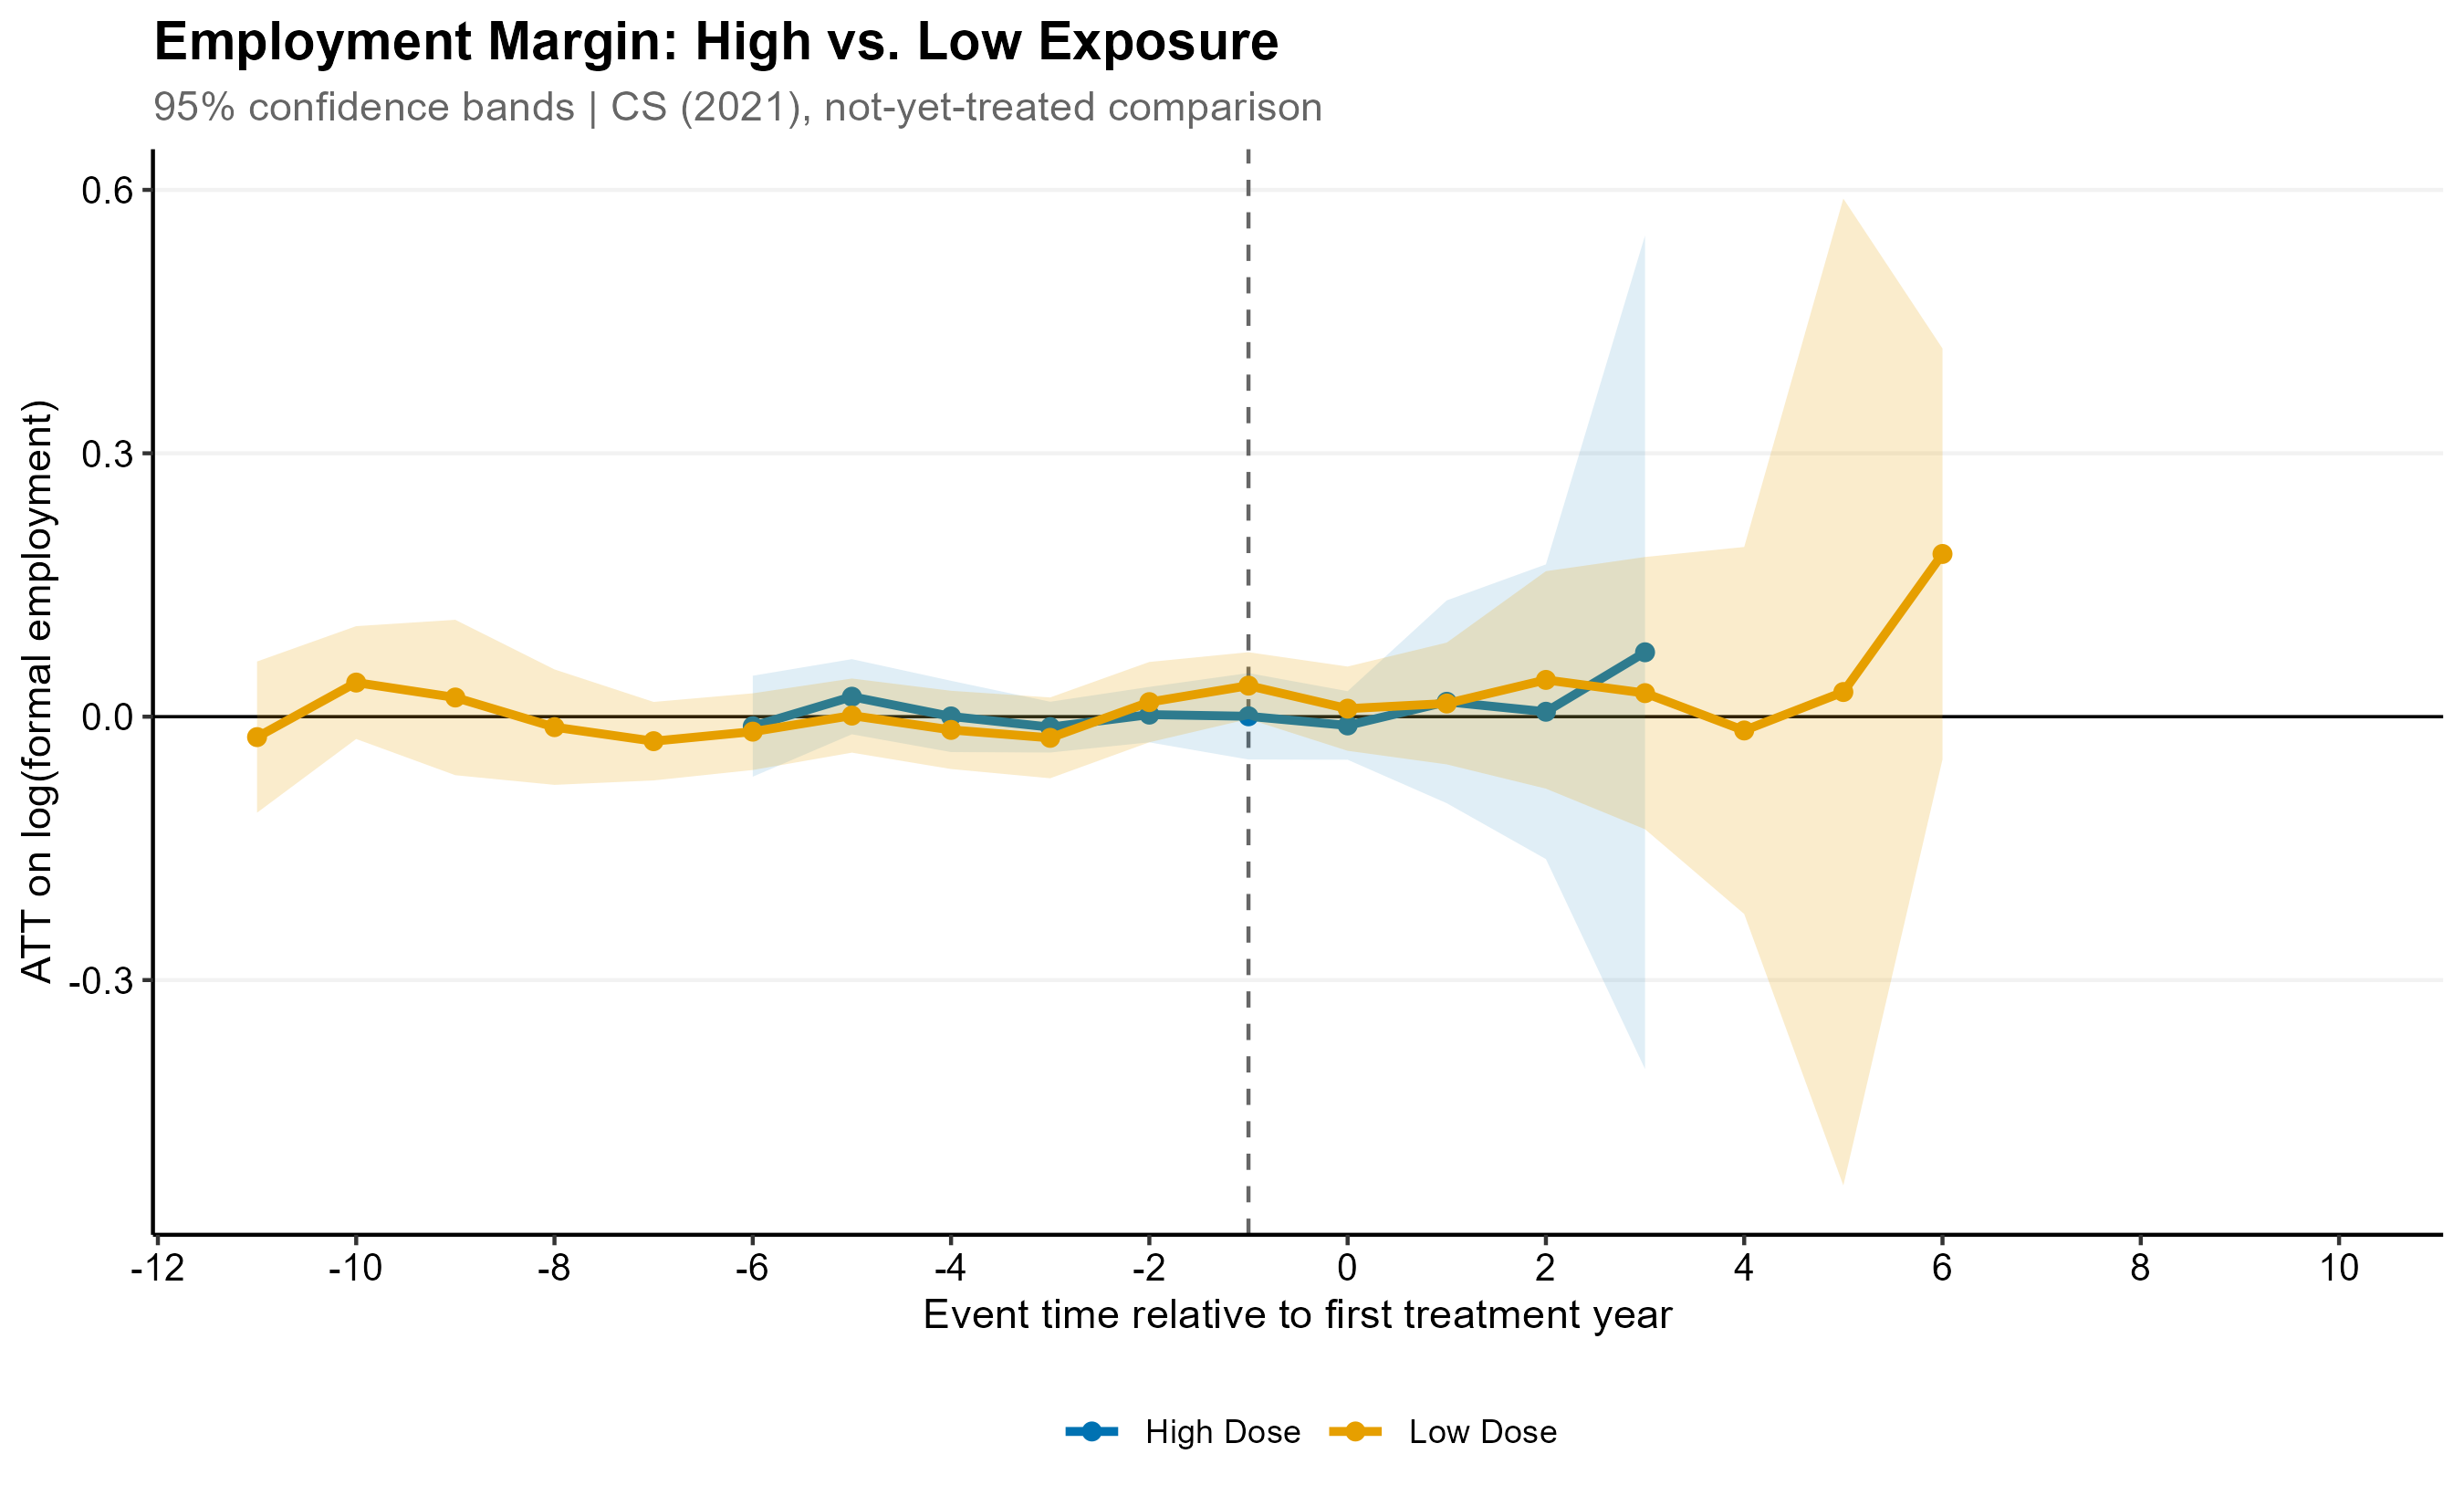
\includegraphics[width=0.85\textwidth]{Figures/fig_3_employment_dose.png}
\caption{\textbf{Employment Margin: High vs.\ Low Exposure.} ATT on log formal employment (v\'inculos, ages 22--35).}
\label{fig:employment}
\end{figure}

The absence of large employment effects is not surprising in a context where RAIS captures only formal employment. ProUni may shift workers from informal to formal jobs without changing the total headcount of 22--35 year-olds, so the employment outcome should be interpreted as a formal-sector extensive-margin measure rather than as a complete labour-market quantity effect.

\subsection{Age-Cohort Decomposition}
\label{sec:cohort_results}

\subsubsection{Headline: Cohort Wage Gap}

To isolate the age-specific human capital channel, I estimate the treatment effect on the within-microregion wage gap between the exposed cohort (ages 22--28) and the control cohort (ages 29--35), as described in Section~\ref{sec:estimation_equations}. Figure~\ref{fig:cohort_gap} reports the results.

\begin{figure}[ht]
\centering
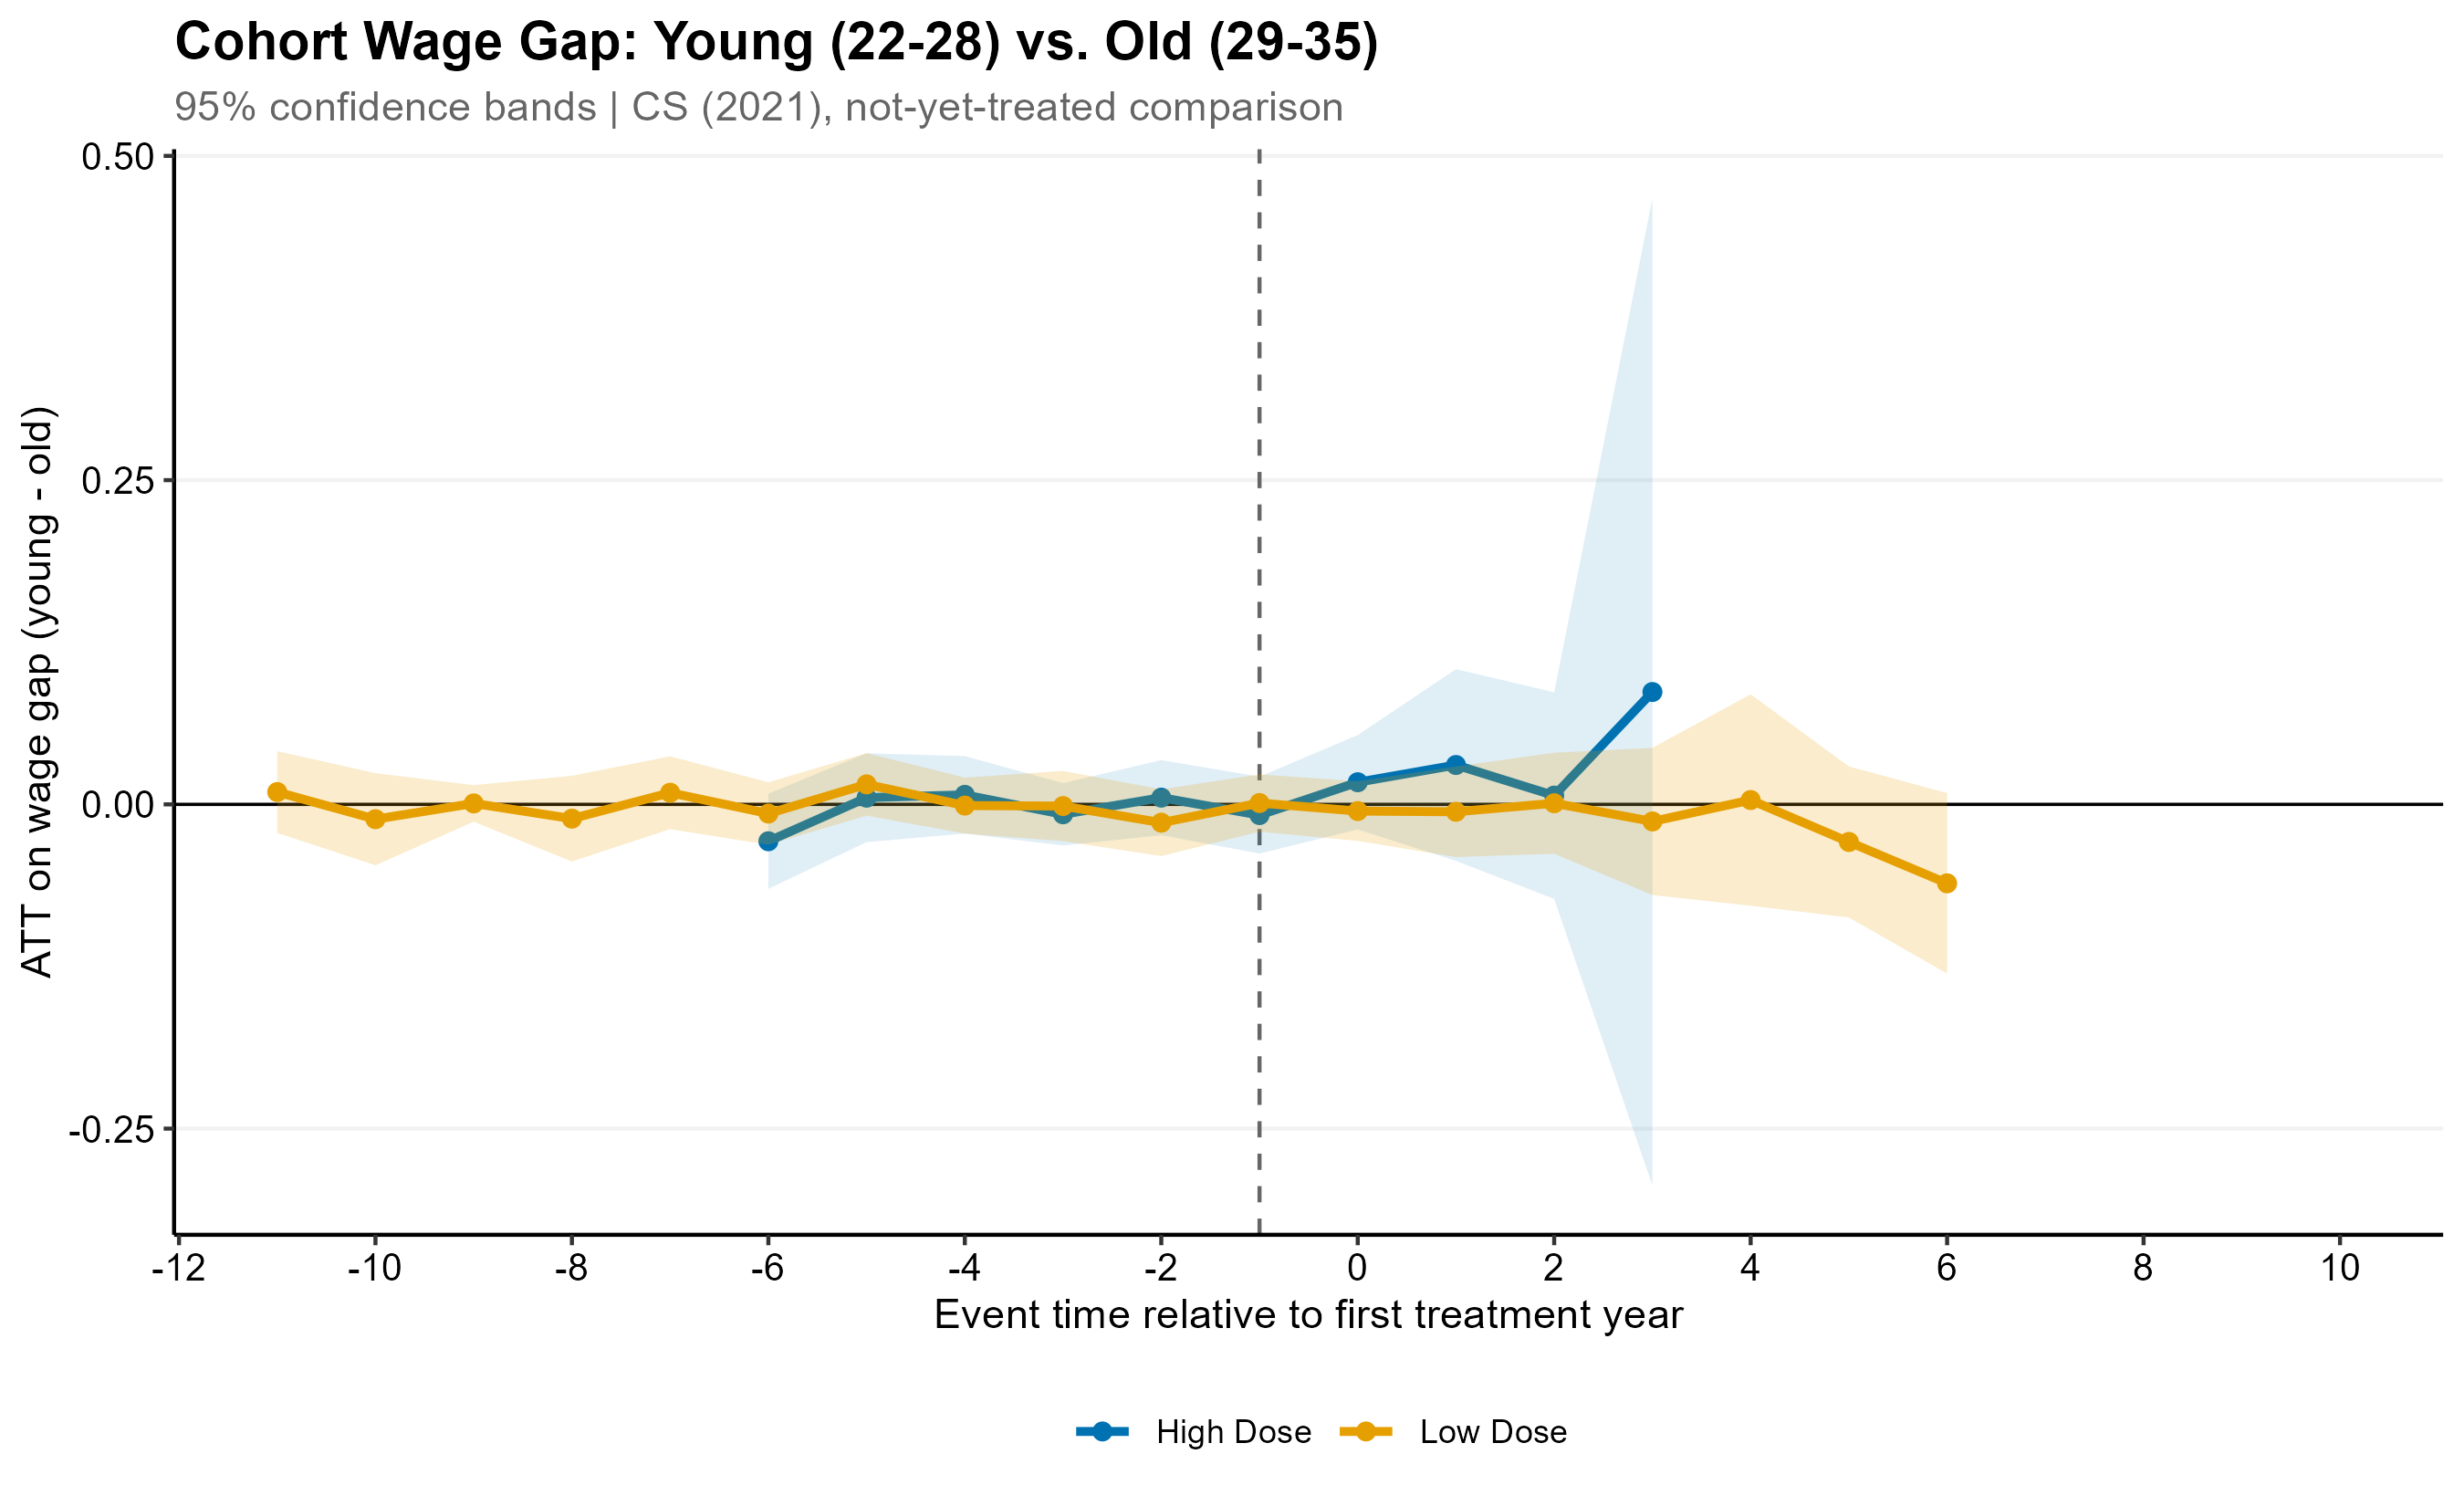
\includegraphics[width=0.85\textwidth]{Figures/fig_cohort_gap.png}
\caption{\textbf{Cohort Wage Gap: Young (22--28) vs.\ Old (29--35).} ATT on the within-microregion wage gap ($\Delta w_{r,t}$). A positive ATT indicates that ProUni raised the relative wage of the young (exposed) cohort.}
\label{fig:cohort_gap}
\end{figure}

The cohort wage-gap results are noisier than the pooled estimates and do not deliver a sharp confirmation of the baseline low-dose pattern. The High-Dose series shows a modest positive drift after treatment (overall ATT of $2.34\%$, $SE = 0.0273$), while the Low-Dose series remains close to zero and slightly negative on average (overall ATT of $-0.54\%$, $SE = 0.0120$). Because the confidence intervals are wide, these estimates are best viewed as diagnostic evidence on mechanisms rather than as stand-alone headline effects.

\subsubsection{Decomposition: Young-Only vs.\ Old-Only}

To understand what drives the cohort wage-gap dynamics, I estimate the ATT separately for each age group. Figures~\ref{fig:young_old_low} and \ref{fig:young_old_high} report these decompositions.

\begin{figure}[ht]
\centering
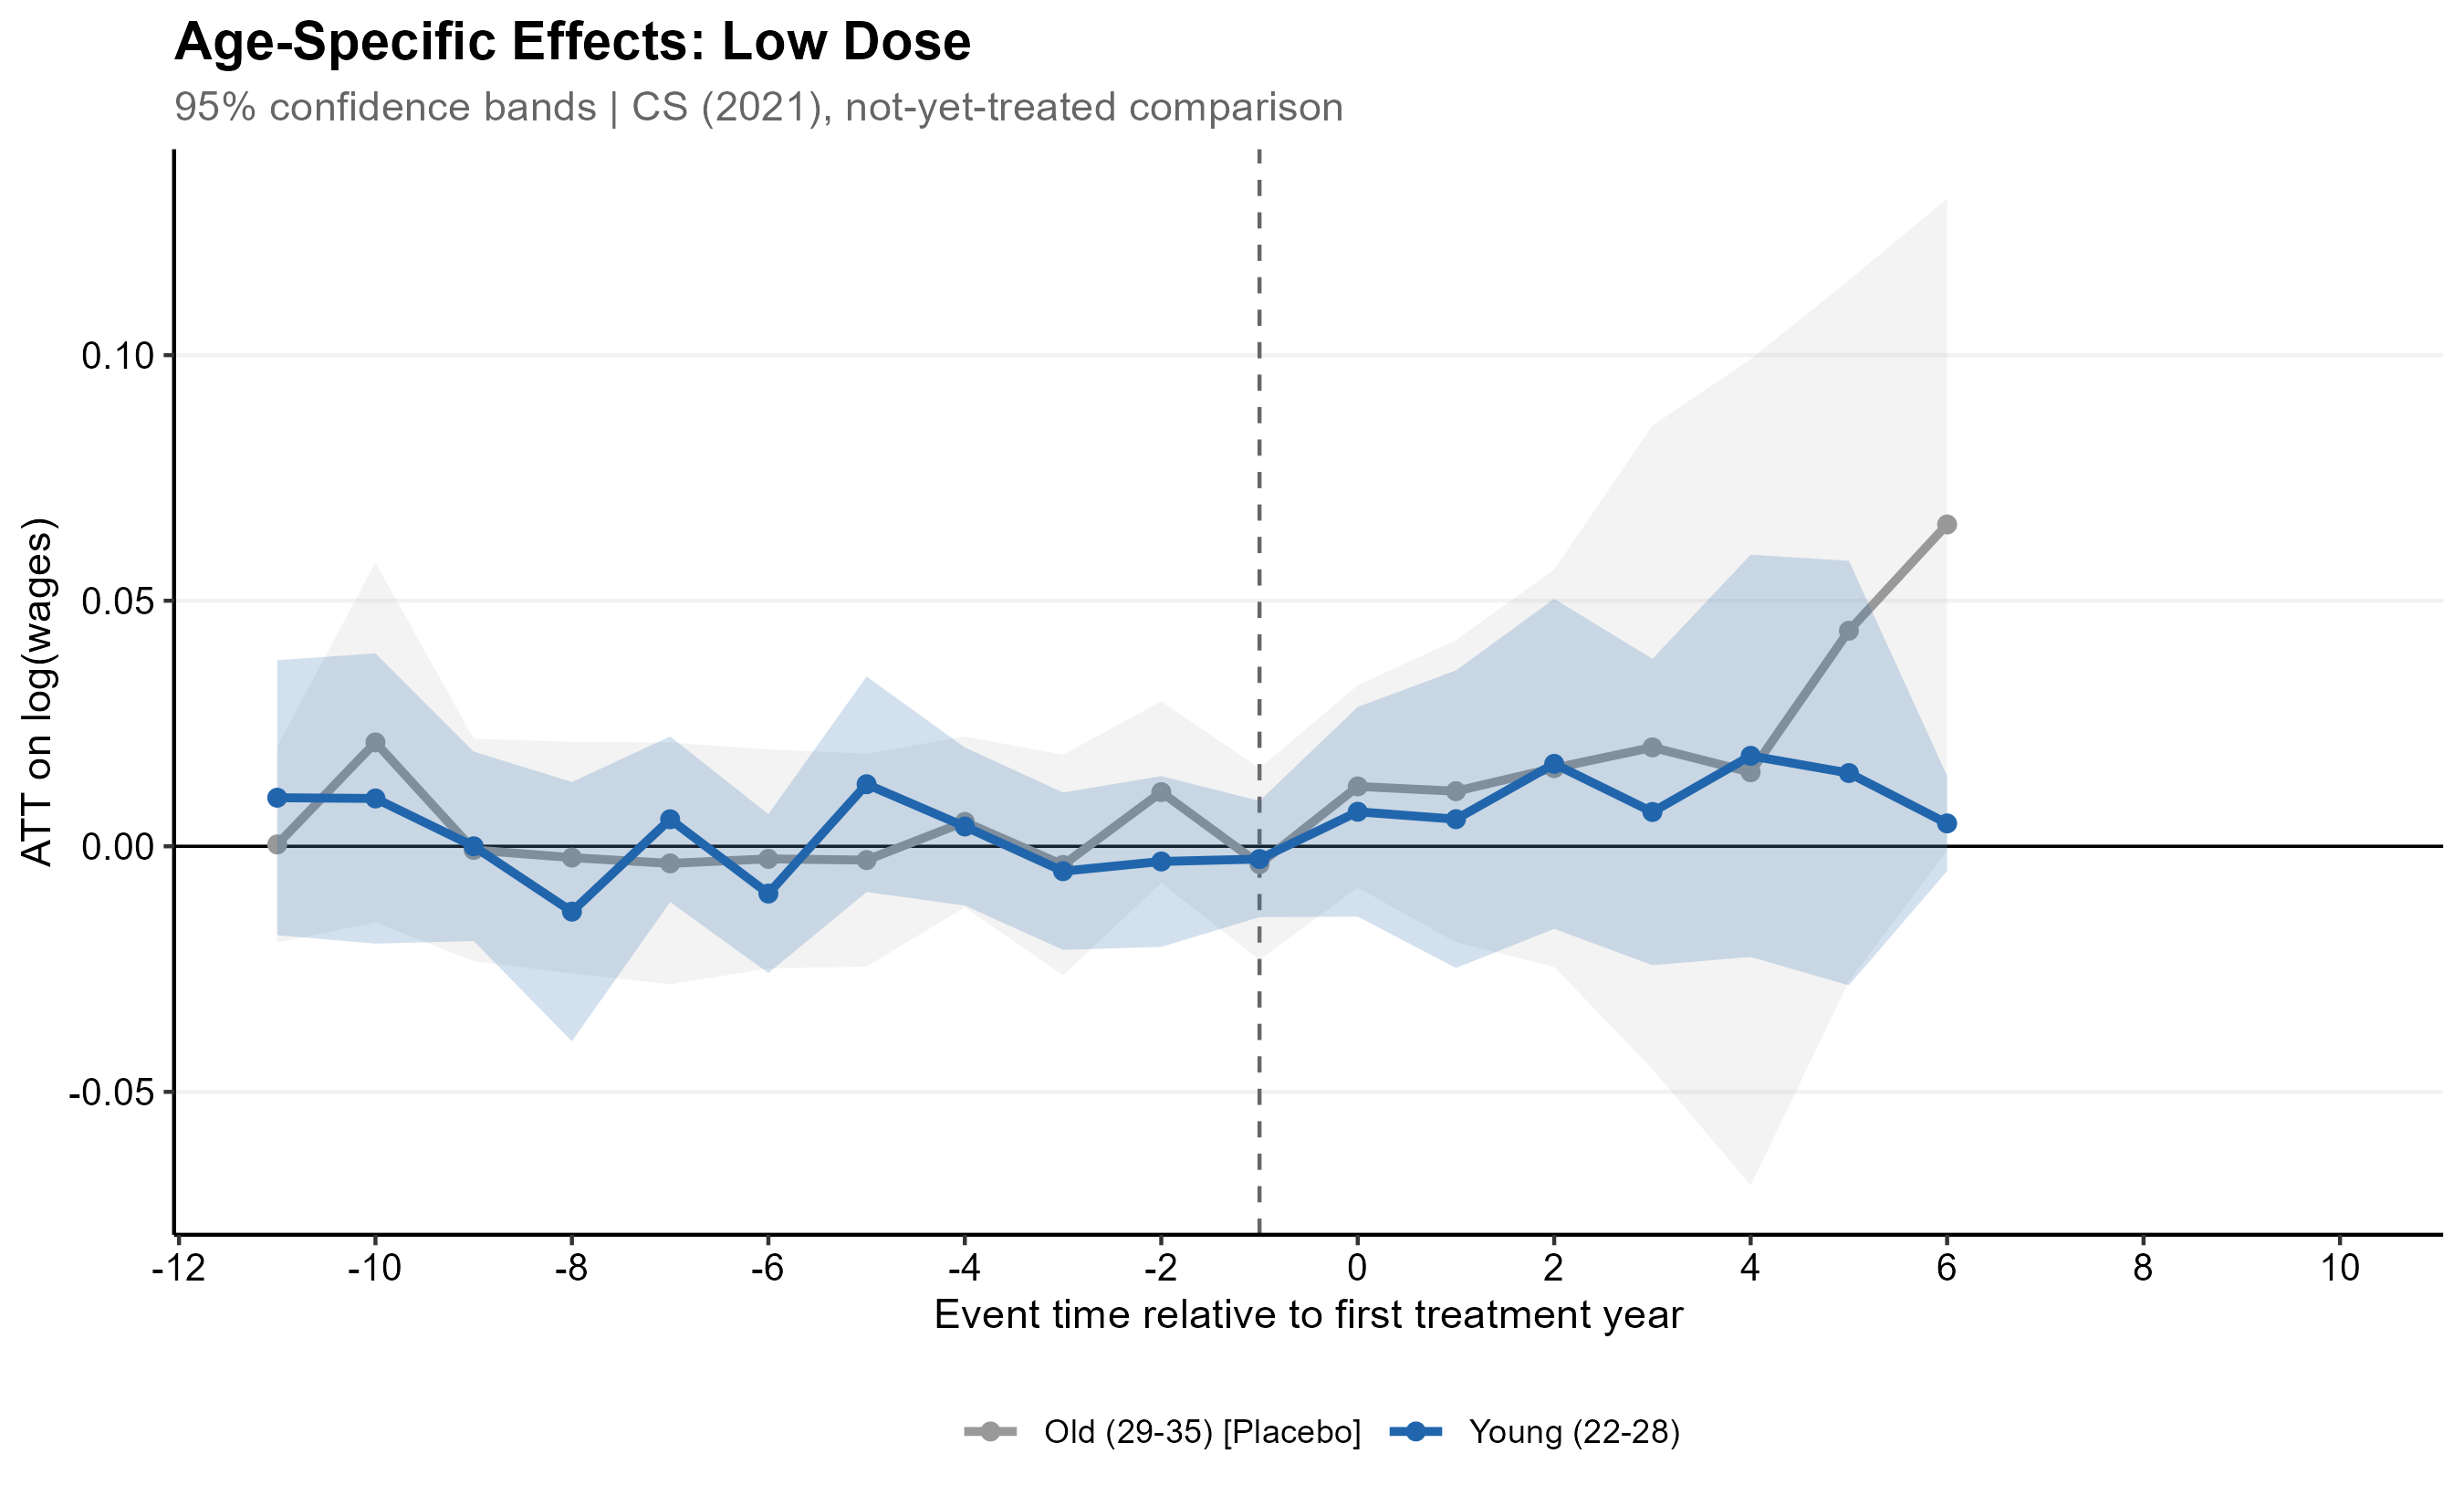
\includegraphics[width=0.85\textwidth]{Figures/fig_cohort_young_vs_old.png}
\caption{\textbf{Age-Specific Effects: Low Dose.} Separate ATTs for young (22--28, exposed) and old (29--35, control cohort).}
\label{fig:young_old_low}
\end{figure}

\begin{figure}[ht]
\centering
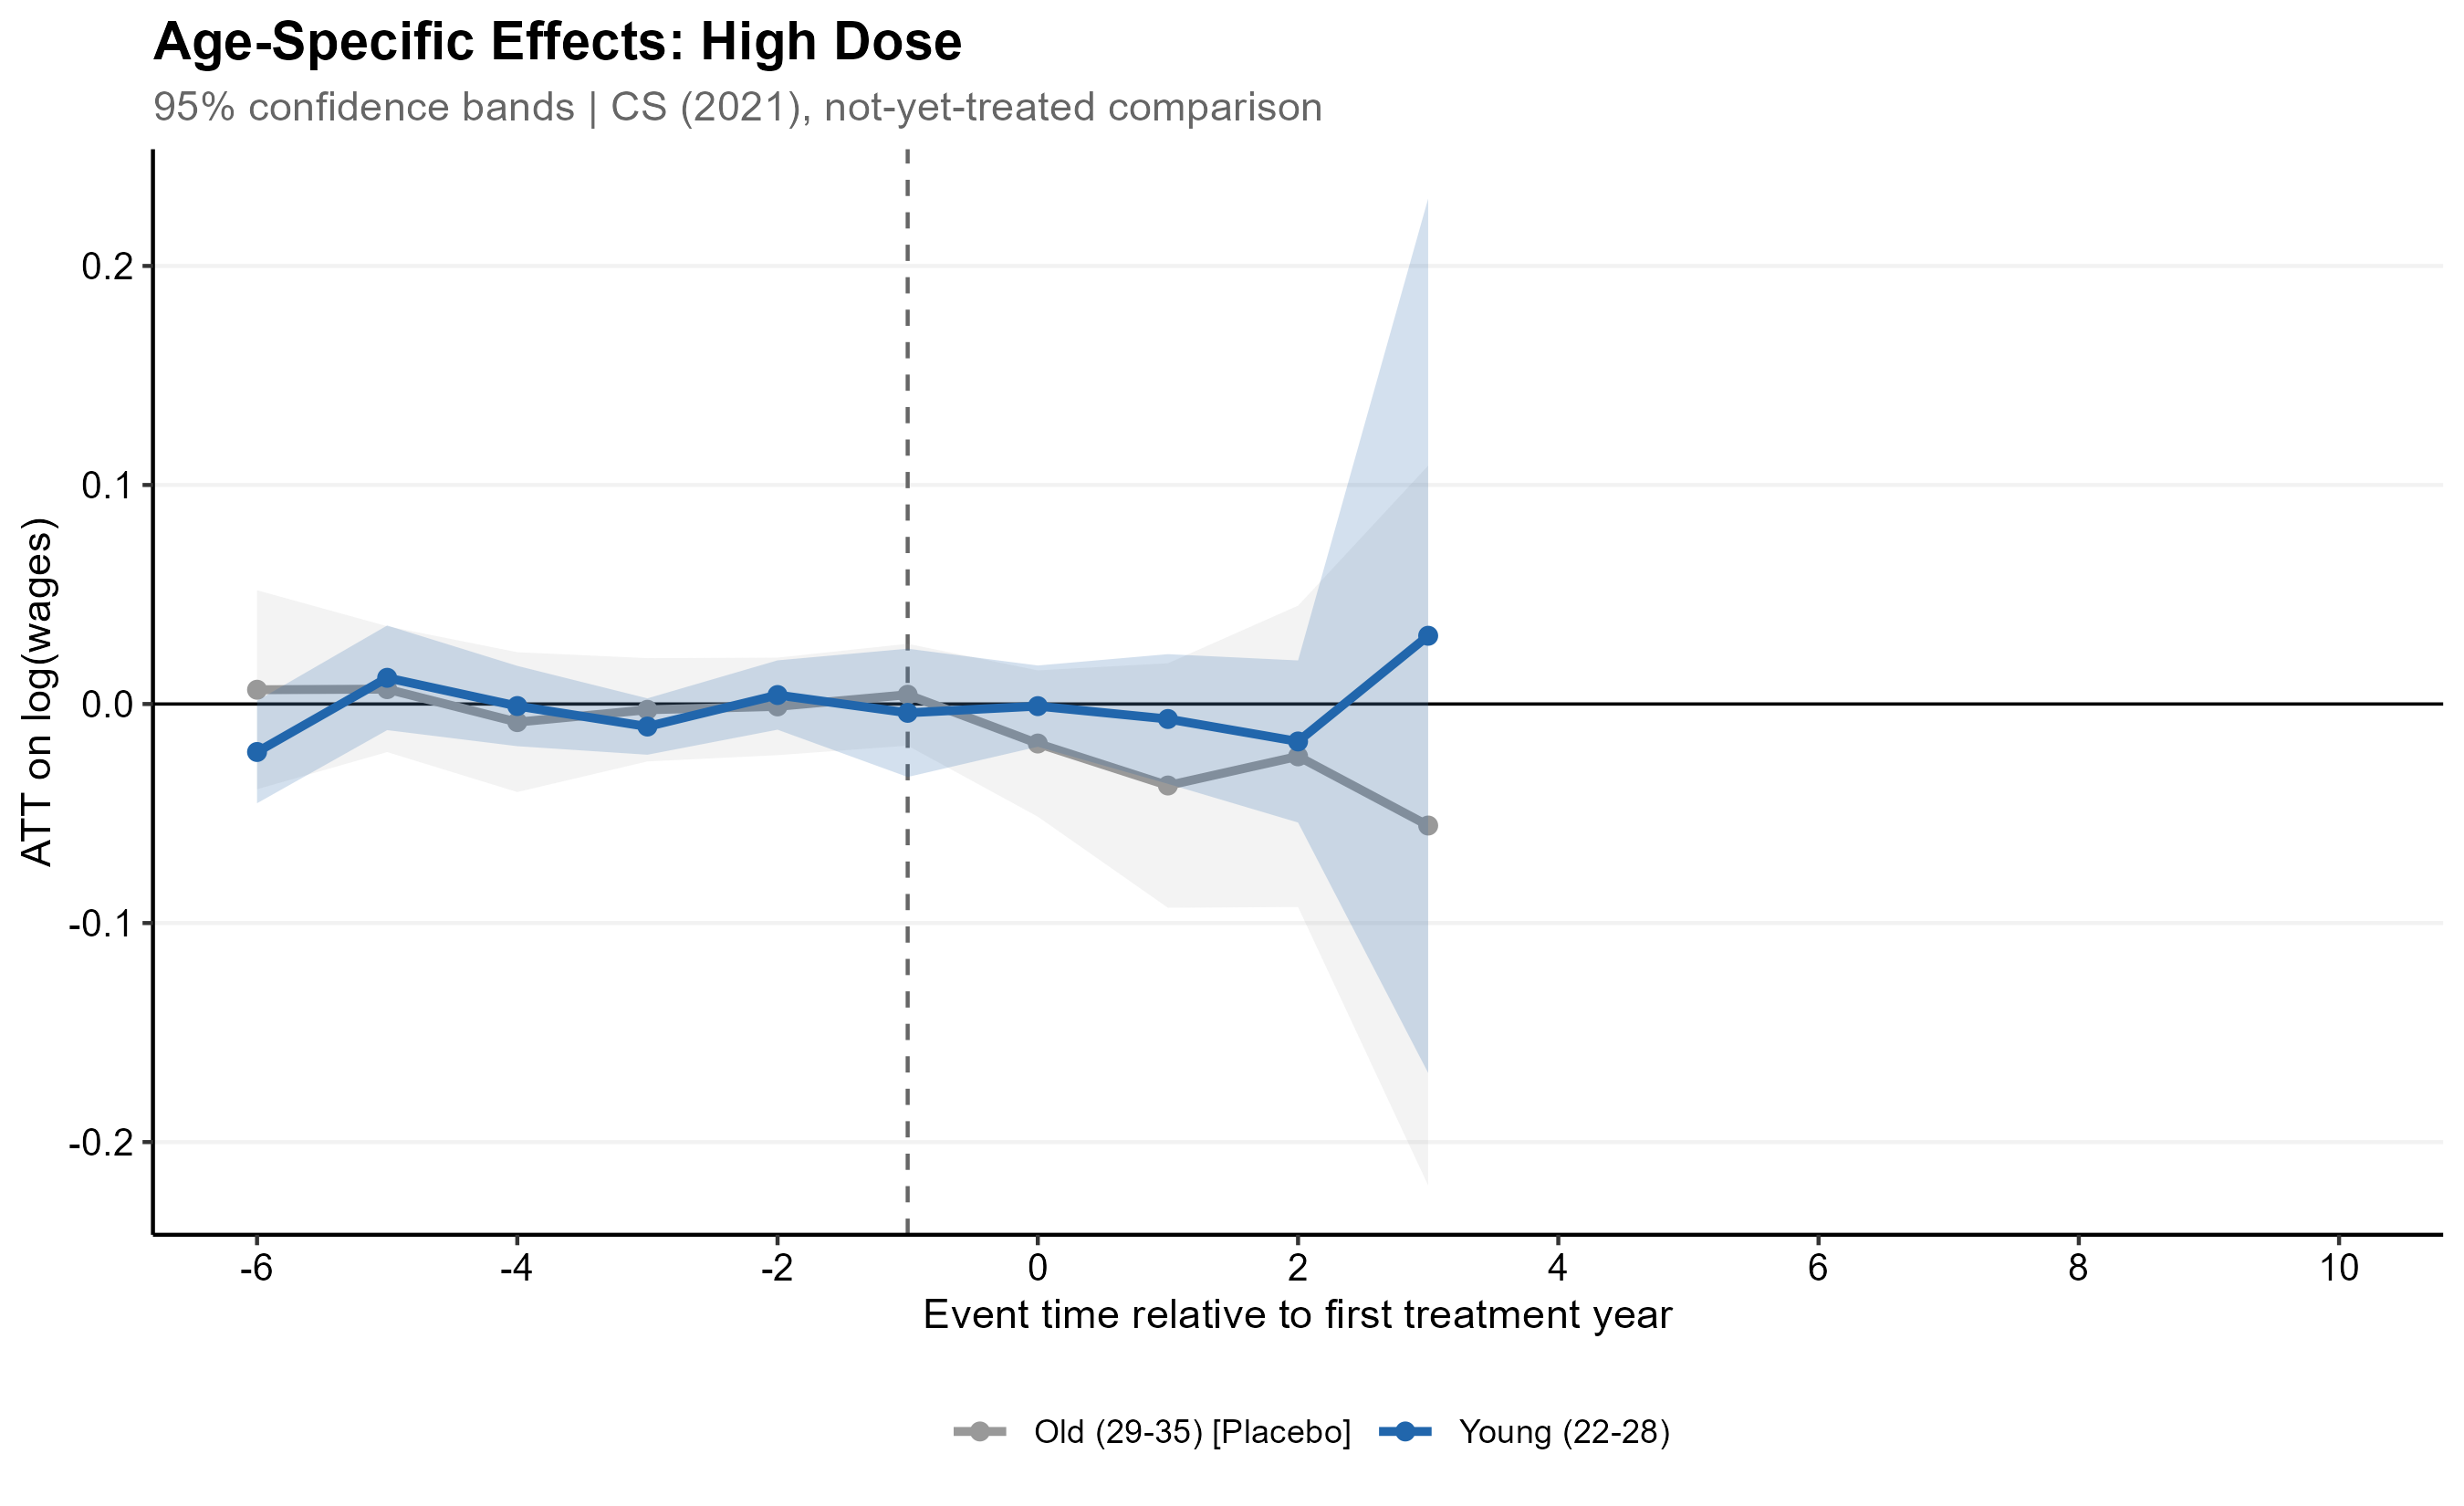
\includegraphics[width=0.85\textwidth]{Figures/fig_cohort_young_vs_old_high.png}
\caption{\textbf{Age-Specific Effects: High Dose.} Separate ATTs for young (22--28) and old (29--35).}
\label{fig:young_old_high}
\end{figure}

The decomposition reveals suggestive but not definitive patterns. In Low-Dose microregions (Figure~\ref{fig:young_old_low}), the young cohort shows a modest positive trajectory, but the old cohort also rises. One interpretation is the presence of positive general-equilibrium spillovers: a moderate inflow of college-educated workers may raise local productivity in a way that benefits multiple age groups. A more cautious alternative is that some residual local shocks correlated with treatment timing remain in the data. The evidence is therefore consistent with spillovers, but it does not mechanically prove them.

In High-Dose microregions (Figure~\ref{fig:young_old_high}), the young cohort remains close to zero while the old cohort declines. This pattern is consistent with displacement or relative wage compression for older workers in heavily exposed markets. At the same time, because the old cohort is intended as a placebo, non-zero effects on that group also warn against an overly mechanical causal interpretation. The decomposition is therefore more informative about plausible mechanisms than about point-identified structural channels.

\subsubsection{First Stage: College Attainment Gap}

Figure~\ref{fig:first_stage} reports the estimated effect of ProUni density on the college share gap between young and old workers.

\begin{figure}[ht]
\centering
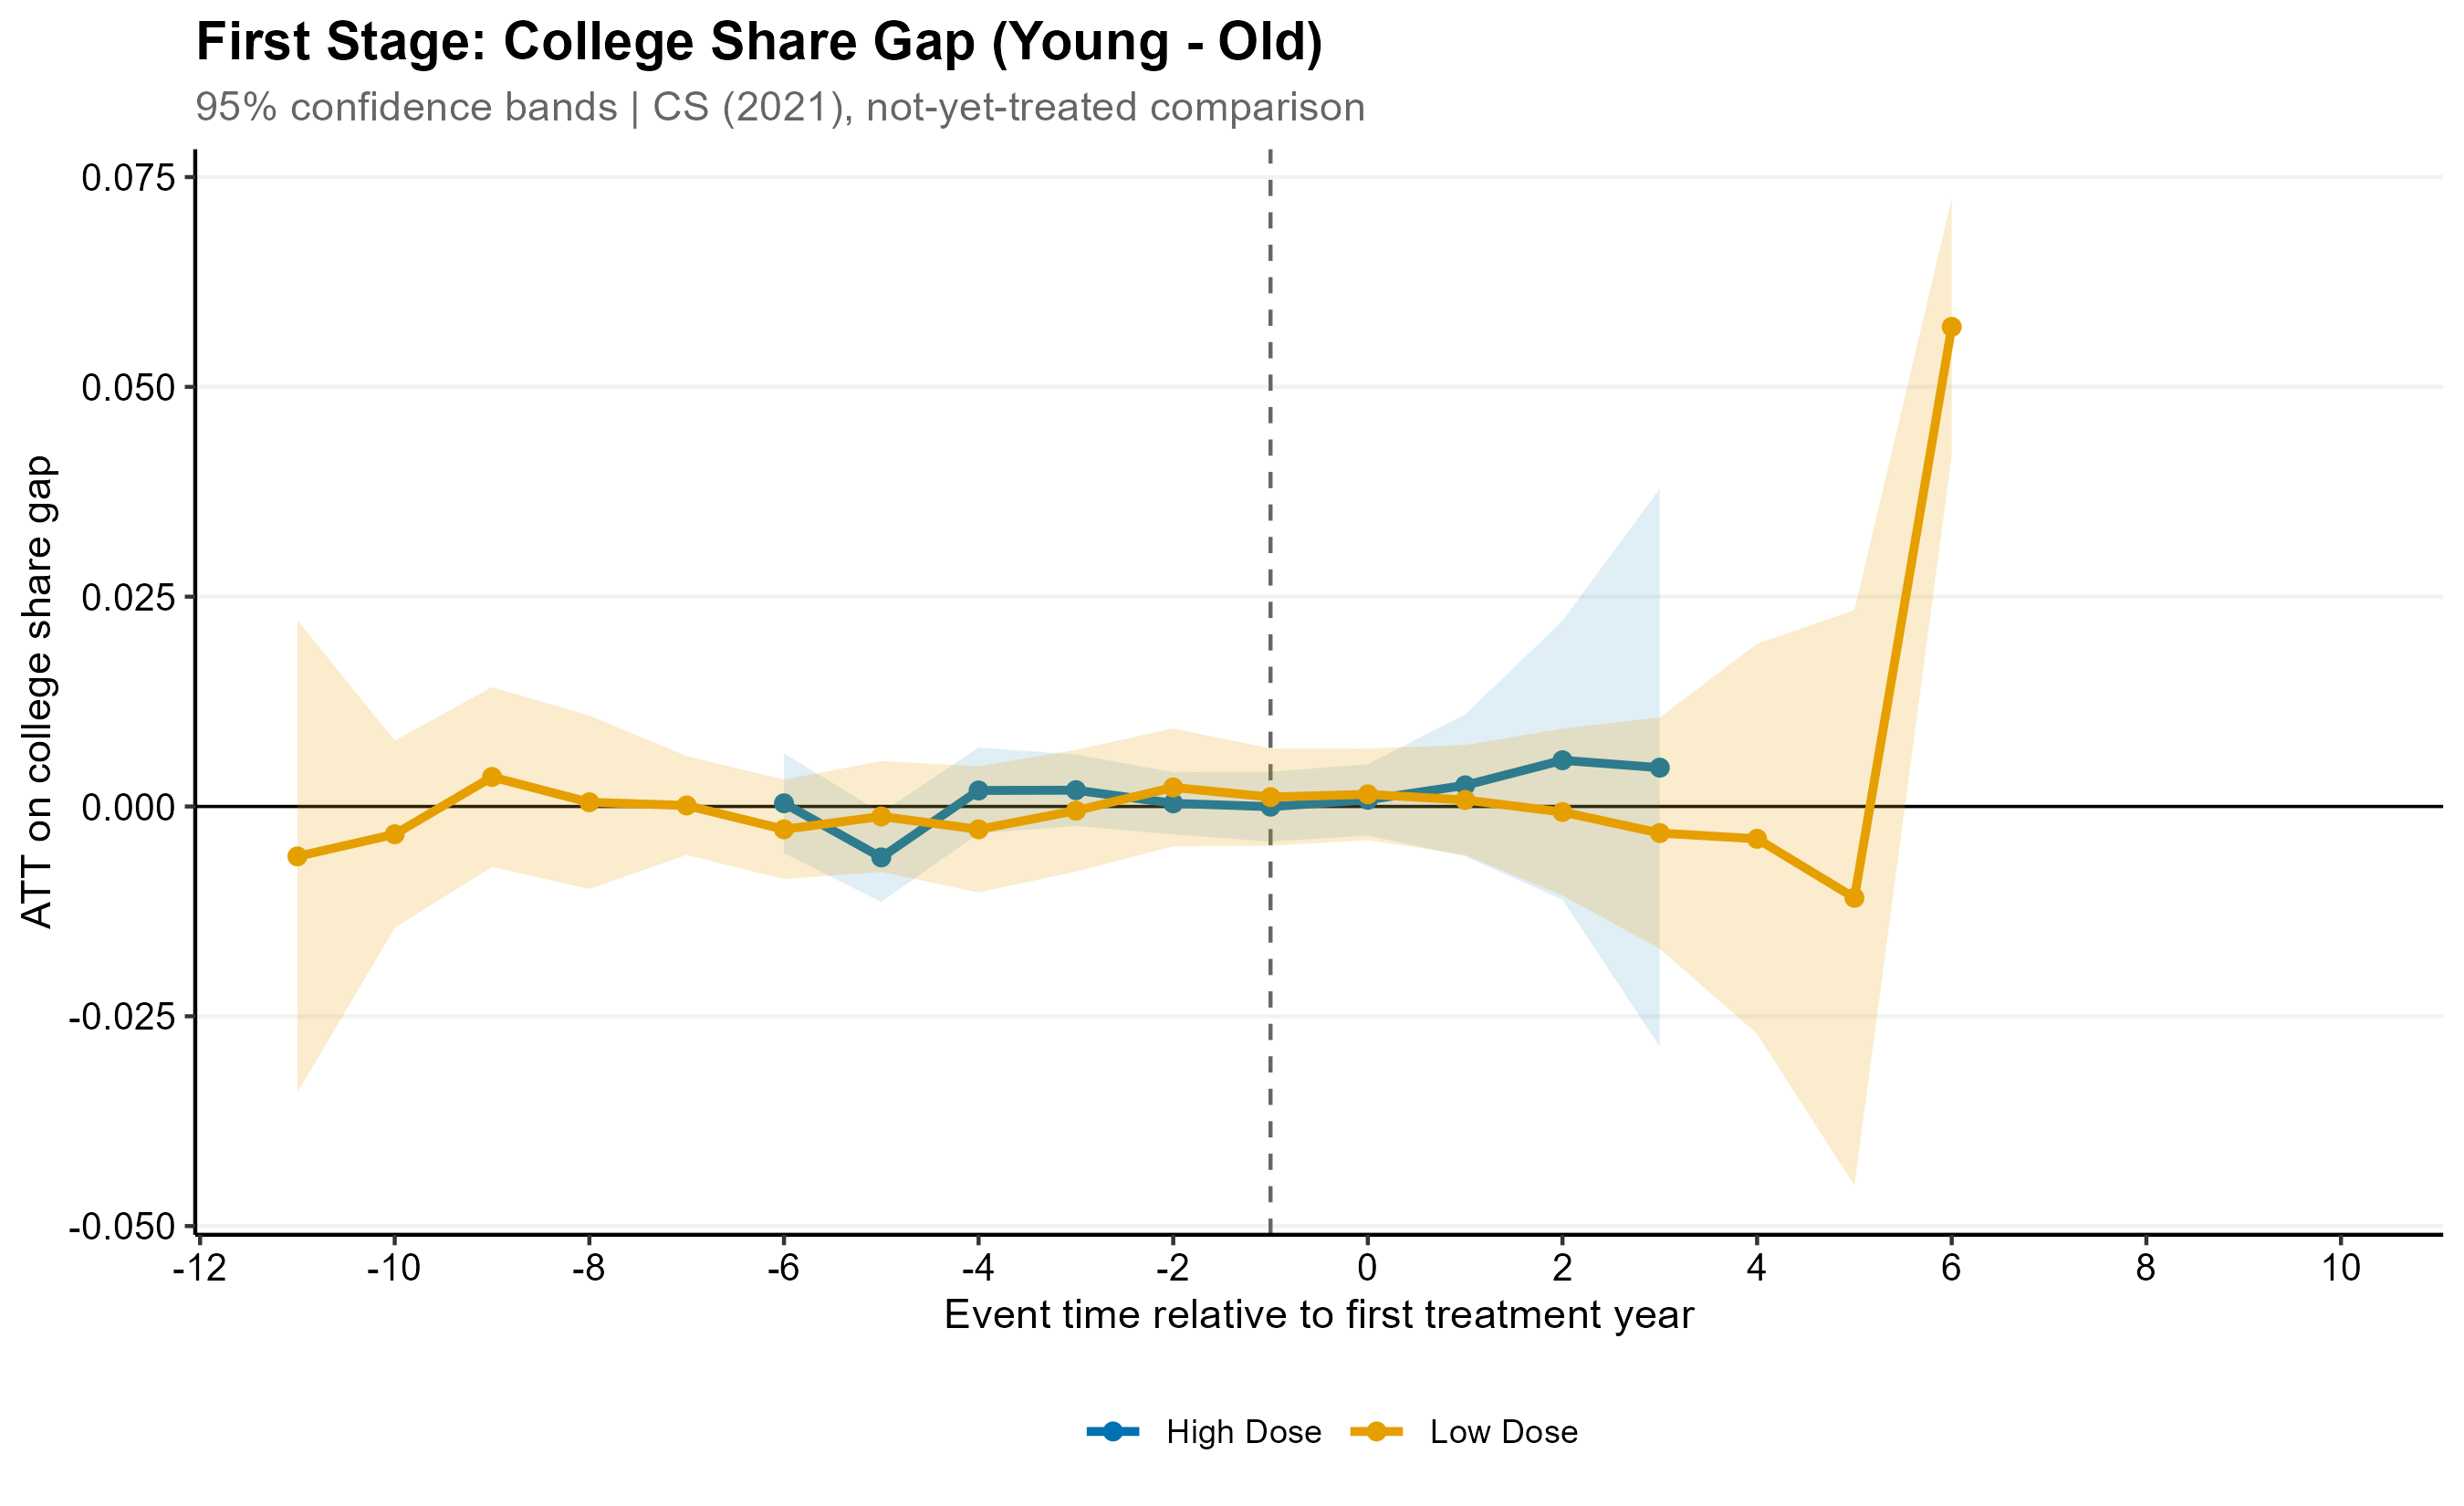
\includegraphics[width=0.85\textwidth]{Figures/fig_first_stage.png}
\caption{\textbf{First Stage: College Share Gap (Young $-$ Old).} ATT on the difference in college-educated worker shares between age cohorts.}
\label{fig:first_stage}
\end{figure}

The first-stage estimates are exceptionally small in magnitude for most post-treatment periods. For High-Dose microregions, the overall ATT is $0.24\%$ ($SE = 0.0031$), while for Low-Dose it is effectively zero. The weakness of the first stage likely reflects both measurement error in employer-reported RAIS education and dilution from computing tertiary shares over the full formal workforce. As a consequence, Wald-style LATE calculations are highly unstable and should not be used as core evidence on the return to a ProUni degree. The thesis therefore relies primarily on reduced-form policy effects.

\subsection{Heterogeneity by Gender and Ethnicity}
\label{sec:heterogeneity}

\subsubsection{Pooled Heterogeneity}

\paragraph{Gender.}
Figure~\ref{fig:gender_pooled} reports the gender-stratified pooled event studies. In Low-Dose microregions, male workers exhibit a positive and growing wage effect (overall ATT $1.67\%$, $SE = 0.0169$), while female workers remain close to zero on average (overall ATT $-0.03\%$, $SE = 0.0007$). In High-Dose microregions, both genders show estimates near zero.

\begin{figure}[ht]
\centering
\begin{minipage}{0.48\textwidth}
    \centering
    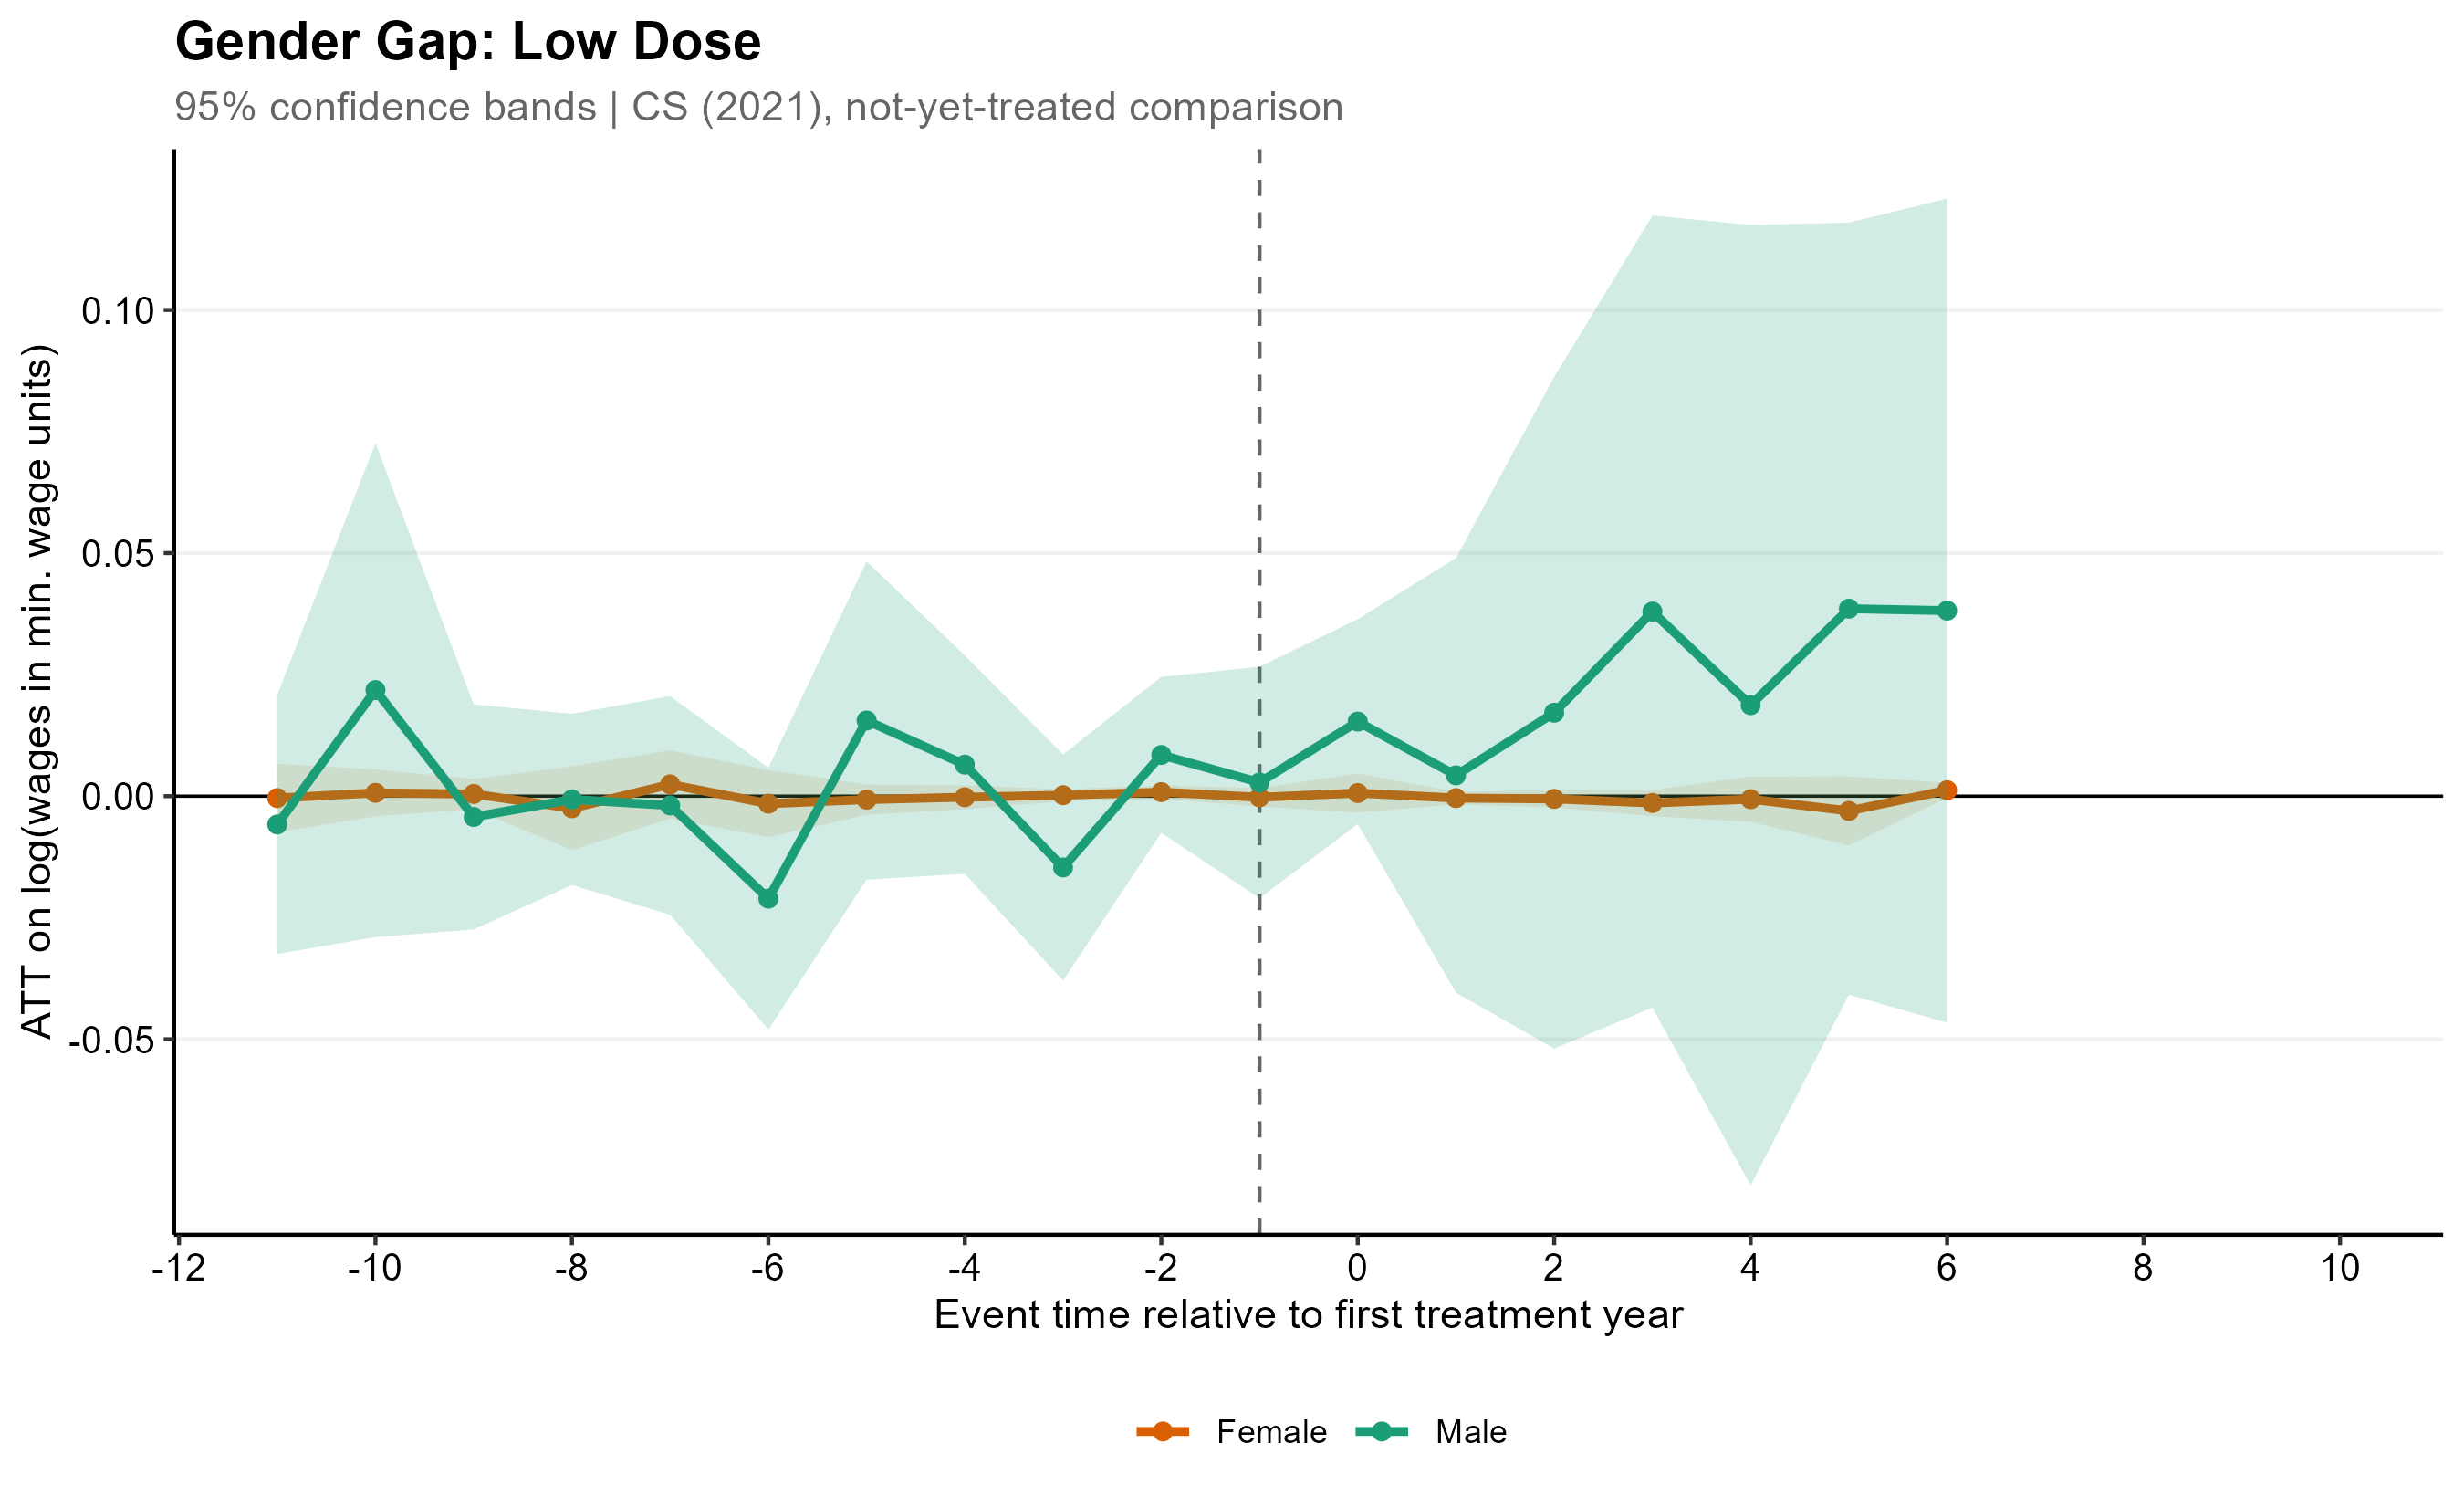
\includegraphics[width=\textwidth]{Figures/fig_4a_gender_low.png}
\end{minipage}
\hfill
\begin{minipage}{0.48\textwidth}
    \centering
    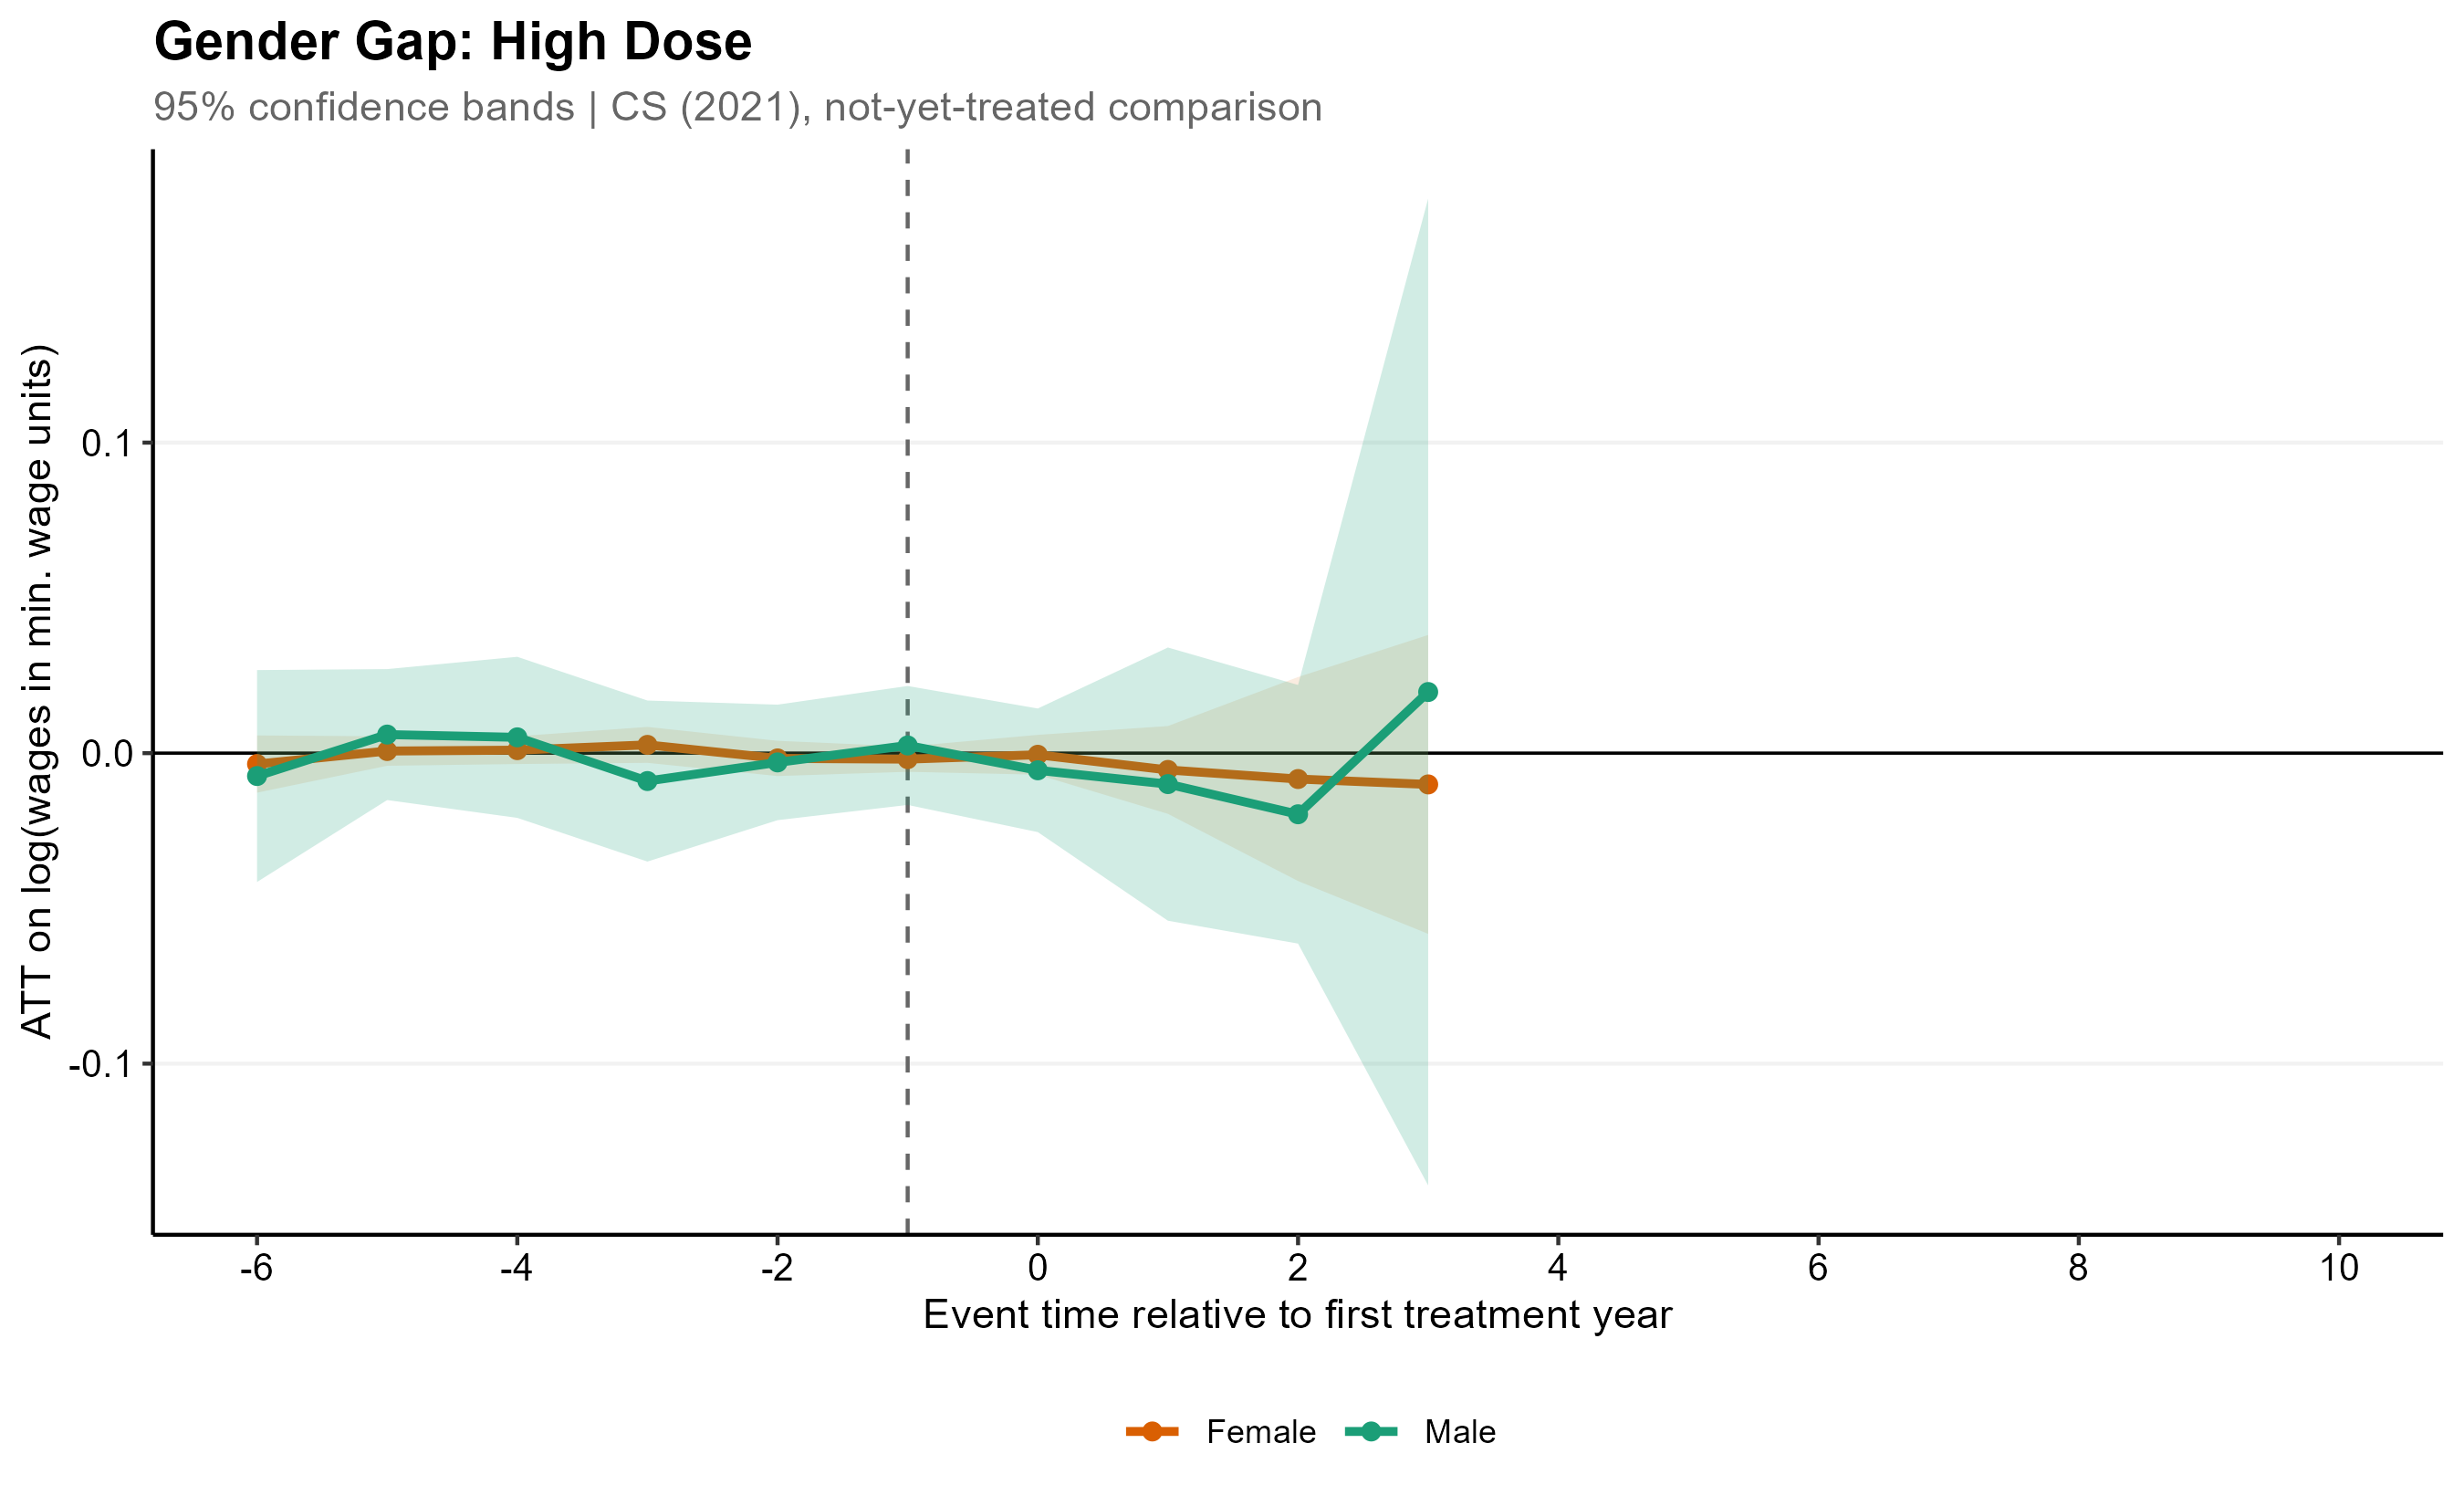
\includegraphics[width=\textwidth]{Figures/fig_4b_gender_high.png}
\end{minipage}
\caption{\textbf{Gender Heterogeneity in Pooled Wage Effects.} Left: Low Dose. Right: High Dose.}
\label{fig:gender_pooled}
\end{figure}

These estimates are consistent with a male wage advantage in the conversion of educational expansion into formal-sector earnings. However, the evidence should be interpreted as reduced-form heterogeneity rather than as direct proof of a single mechanism such as field sorting, discrimination, or labour-force attachment.

\paragraph{Ethnicity.}
Figure~\ref{fig:race_pooled} shows that in Low-Dose microregions, non-white workers exhibit positive trajectories (overall ATT $1.28\%$, $SE = 0.0119$), while white workers remain close to zero on average (overall ATT $-0.22\%$, $SE = 0.0088$). In High-Dose microregions, both groups again show near-zero effects.

\begin{figure}[ht]
\centering
\begin{minipage}{0.48\textwidth}
    \centering
    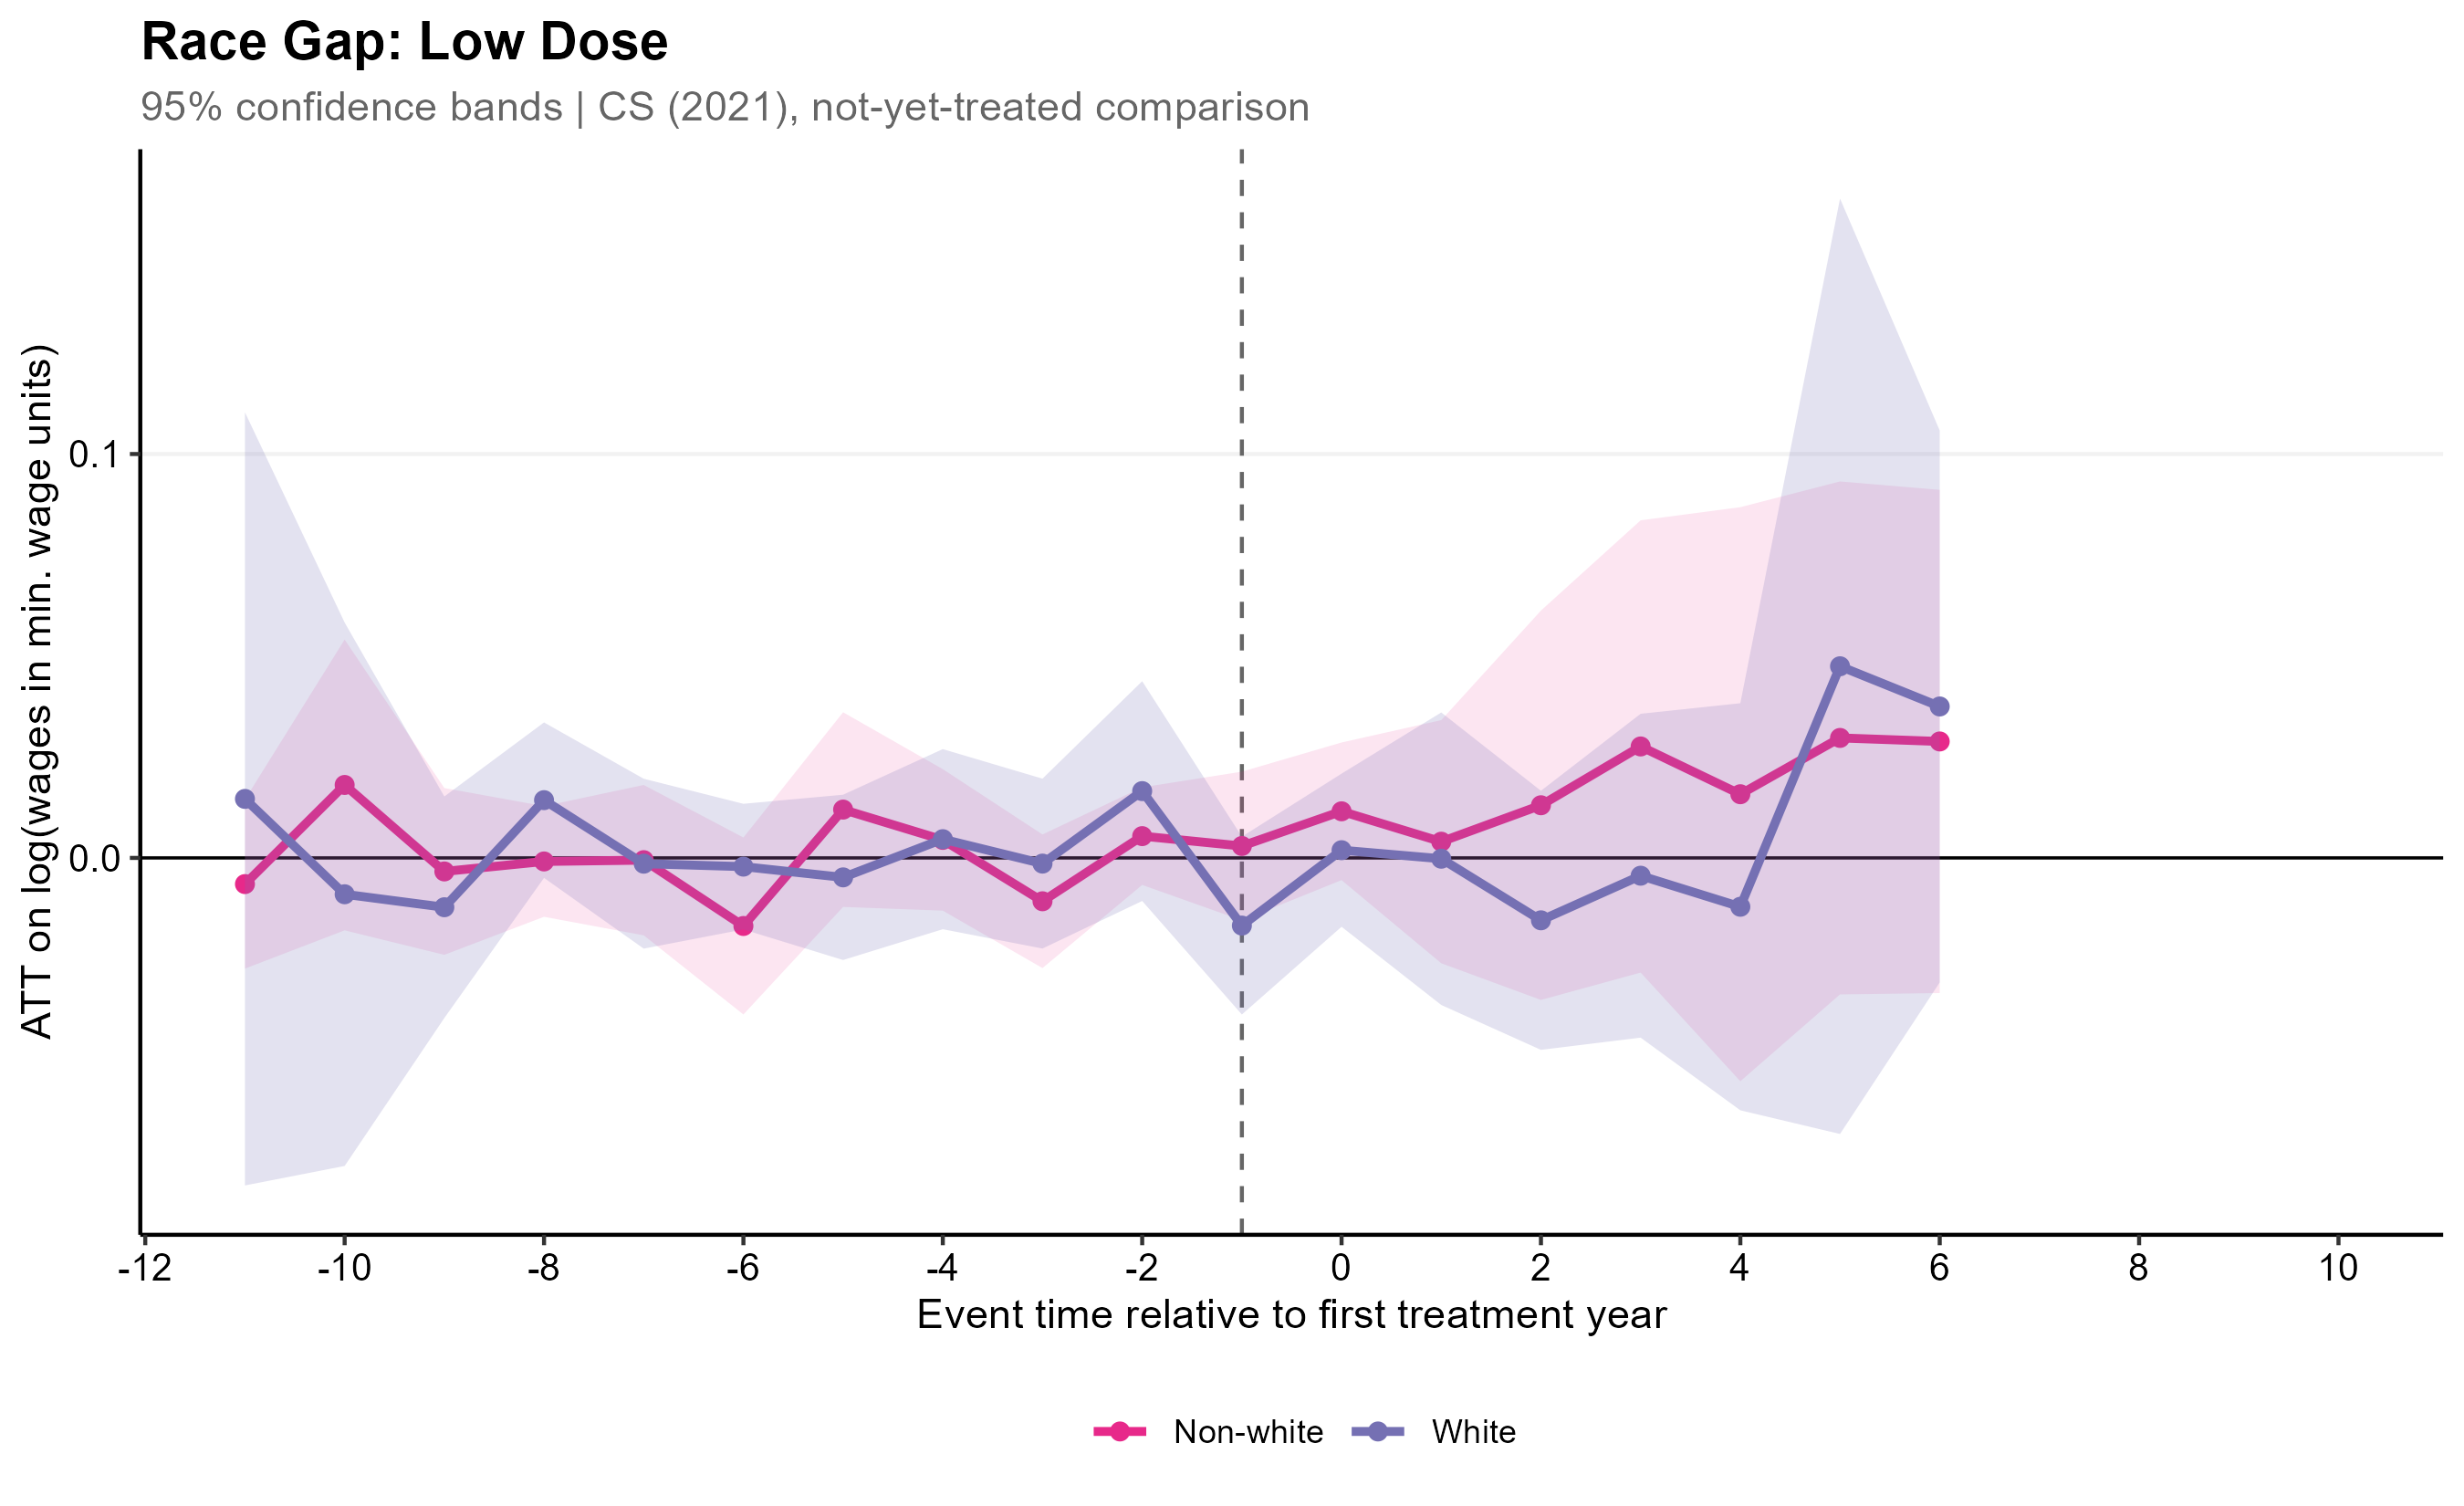
\includegraphics[width=\textwidth]{Figures/fig_5a_race_low.png}
\end{minipage}
\hfill
\begin{minipage}{0.48\textwidth}
    \centering
    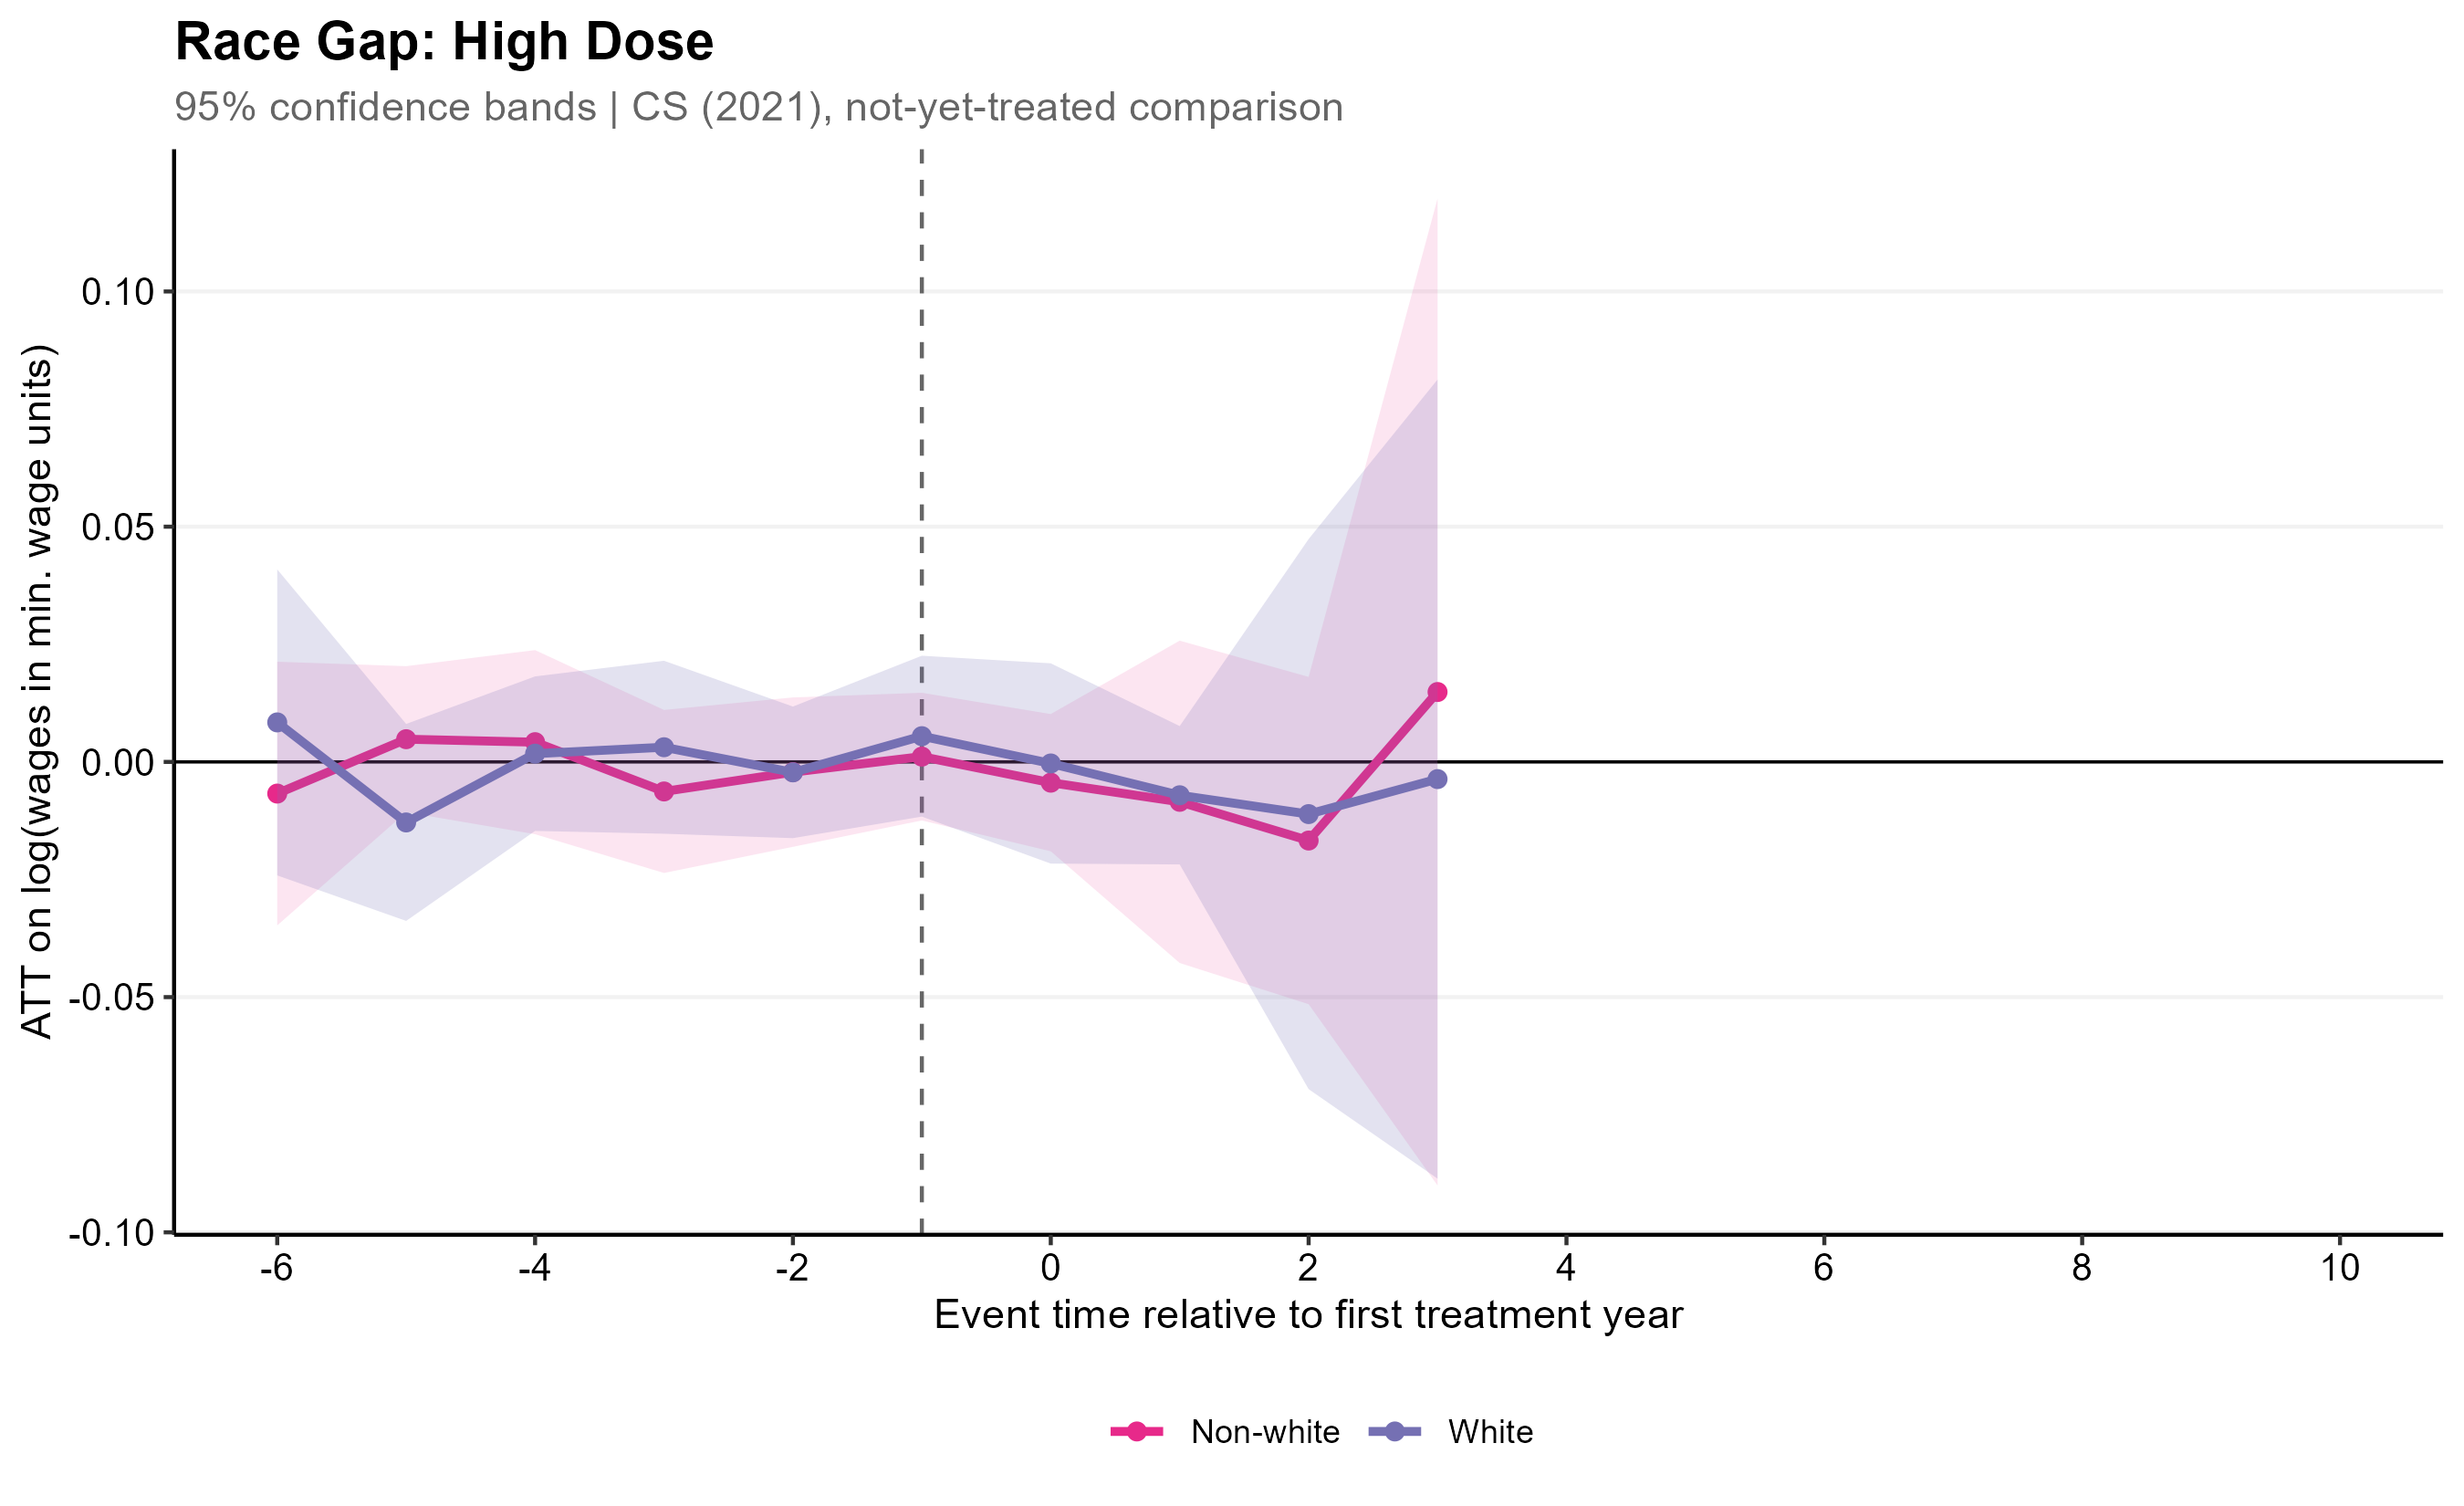
\includegraphics[width=\textwidth]{Figures/fig_5b_race_high.png}
\end{minipage}
\caption{\textbf{Ethnicity Heterogeneity in Pooled Wage Effects.} Left: Low Dose. Right: High Dose.}
\label{fig:race_pooled}
\end{figure}

These patterns are consistent with ProUni improving formal-sector wage outcomes for non-white workers in moderately exposed markets. Even so, the thesis cannot claim full distributive parity or a complete elimination of structural disadvantage on the basis of these reduced-form estimates alone.

\subsection{Robustness Checks}
\label{sec:robustness_results}

\subsubsection{Continuous TWFE and Omitted Variable Bias}

To test whether the High-Dose penalty is confounded by macroeconomic geography, I estimate a sequence of continuous-treatment TWFE models interacting the continuous dosage measure $D_{r,t}$ with a post-treatment dummy for the non-white subsample.

Table~\ref{tab:continuous_twfe} summarizes the results. An unconditional linear specification (Model 1) yields a marginally significant negative dose-response coefficient ($\beta = -0.00013$, $p = 0.0539$). A logarithmic transformation of the dose (Model 2) provides a somewhat better fit ($\beta = -0.0021$, $p = 0.0480$), suggesting diminishing marginal returns as exposure rises. A quadratic specification (Model 3) shows a significant negative linear term but an insignificant squared term ($p = 0.3131$), offering no evidence of recovery at extreme saturation levels.

However, once the TWFE model is augmented with baseline covariates interacted with the post-treatment dummy (Model 4), the direct effect of ProUni dose disappears ($p = 0.3699$). The interaction between post-treatment timing and baseline household income per capita is large, negative, and statistically significant ($\beta = -0.0377$, $p = 0.0015$). This suggests that unconditional high-dose penalties partly load onto the adverse macroeconomic shocks experienced by Brazil's wealthier economic hubs during the 2014--2016 recession, rather than cleanly isolating a pure educational saturation effect.

\begin{table}[ht]
\centering
\caption{\textbf{Continuous TWFE Models: Testing for Saturation and OVB}}
\label{tab:continuous_twfe}
\begin{tabular}{lcccc}
\hline
 & \textbf{Linear (1)} & \textbf{Log (2)} & \textbf{Quadratic (3)} & \textbf{Covariates (4)} \\
\hline
$D_{r,t} \times \text{post}$ & -0.0001$^{*}$ &  & -0.0003$^{**}$ & 0.00007 \\
 & (0.0001) &  & (0.0001) & (0.0001) \\
$\ln(1 + D_{r,t}) \times \text{post}$ &  & -0.0021$^{**}$ &  &  \\
 &  & (0.0011) &  &  \\
$D_{r,t}^2 \times \text{post}$ &  &  & 0.000001 &  \\
 &  &  & (0.000001) &  \\
Avg. HH Income $\times \text{post}$ &  &  &  & -0.0377$^{***}$ \\
 &  &  &  & (0.0118) \\
\hline
Observations & 7,812 & 7,812 & 7,812 & 7,812 \\
Microregion \& Year FEs & Yes & Yes & Yes & Yes \\
\hline
\multicolumn{5}{l}{\small Standard errors clustered by microregion in parentheses. $^{*} p<0.10$, $^{**} p<0.05$, $^{***} p<0.01$.}
\end{tabular}
\end{table}

\subsubsection{TWFE Benchmark vs. Callaway-Sant'Anna}

Table~\ref{tab:twfe} compares the naive binary TWFE estimates with the \citeA{CallawaySantAnna2021} ATTs. The TWFE wage coefficient is $-0.65\%$ ($SE = 0.0037$), masking the positive low-dose estimate and mechanically pooling heterogeneous cohort-time comparisons. This divergence confirms that a single pooled TWFE coefficient is not an informative summary of the underlying staggered design.

\begin{table}[ht]
\centering
\caption{\textbf{TWFE vs.\ Callaway-Sant'Anna Comparison}}
\label{tab:twfe}
\begin{tabular}{lccc}
\hline
\textbf{Specification} & \textbf{ATT} & \textbf{SE} & \textbf{N} \\
\hline
TWFE / Wages (pooled)       & -0.0065 & 0.0037 & 7,812 \\
CS / Low Dose (wages)       & 0.0128 & 0.0128 & 3,906 \\
CS / High Dose (wages)      & -0.0070 & 0.0074 & 3,528 \\
TWFE / Wage Gap (cohort)    & 0.0072 & 0.0042 & 7,810 \\
CS / Gap Low                & -0.0054 & 0.0120 & 3,904 \\
CS / Gap High               & 0.0234 & 0.0273 & 3,526 \\
\hline
\end{tabular}
\end{table}

\subsection{Summary of Findings}

Table~\ref{tab:master_summary} consolidates the key estimates across primary models.

\begin{table}[ht]
\centering
\caption{\textbf{Summary of Main ATT Estimates}}
\label{tab:master_summary}
\begin{tabular}{lccccc}
\hline
\textbf{Model} & \textbf{ATT} & \textbf{SE} & \textbf{95\% CI} & \textbf{p-value (pre-trend)} & \textbf{N (obs)} \\
\hline
\textit{Pooled Wages} & & & & & \\
Low Dose & 0.0128 & 0.0128 & [-0.012, 0.038] & 0.359 & 3,906 \\
High Dose & -0.0070 & 0.0074 & [-0.022, 0.008] & 0.916 & 3,528 \\
Low Dose (DR) & 0.0259 & 0.0145 & [-0.003, 0.054] & 0.535 & 3,906 \\
\hline
\textit{Cohort Wage Gap} & & & & & \\
Low Dose & -0.0054 & 0.0120 & [-0.029, 0.018] & 0.707 & 3,904 \\
High Dose & 0.0234 & 0.0273 & [-0.030, 0.077] & 0.539 & 3,526 \\
\hline
\textit{Employment} & & & & & \\
Low Dose & 0.0182 & 0.0332 & [-0.047, 0.083] & 0.120 & 3,906 \\
High Dose & 0.0065 & 0.0396 & [-0.071, 0.084] & 0.809 & 3,528 \\
\hline
\end{tabular}
\end{table}

Taken together, the results support four disciplined conclusions. First, within Low-Dose microregions, the reduced-form wage estimates are positive and economically meaningful, though statistically imprecise. Second, estimated gains are weaker in High-Dose markets, but the interpretation of that difference as causal saturation is fragile because it is sensitive to controls for macroeconomic geography and requires stronger identifying assumptions. Third, the age-cohort decomposition suggests that spillovers and relative wage compression are plausible mechanisms, but it does not isolate them with certainty. Fourth, the heterogeneity results are consistent with benefits for non-white workers in moderate-exposure markets and with a persistent male advantage in the translation of educational expansion into formal-sector wages.
